\documentclass[11pt,a4paper]{article}
\usepackage{fontspec}
\setmonofont{DejaVu Sans Mono}[Scale=0.85]
\usepackage[margin=2.3cm]{geometry}
\usepackage{xcolor}
\usepackage{listings}
\usepackage[most]{tcolorbox}
\usepackage{enumitem}
\usepackage{titlesec}
\usepackage{fancyhdr}
\usepackage{booktabs}
\usepackage{tikz}
\usetikzlibrary{arrows.meta,positioning}
\usepackage{array}
\usepackage[hidelinks]{hyperref}

\renewcommand{\contentsname}{Contenido}
\renewcommand{\figurename}{Figura}
\renewcommand{\tablename}{Tabla}

\definecolor{reactblue}{HTML}{087EA4}
\definecolor{reactdark}{HTML}{23272F}
\definecolor{codebg}{HTML}{F6F7F9}
\definecolor{kw}{HTML}{C0306F}
\definecolor{str}{HTML}{2E7D32}
\definecolor{com}{HTML}{7A7F87}
\definecolor{warn}{HTML}{B45309}
\definecolor{ok}{HTML}{15803D}

\hypersetup{colorlinks=true,linkcolor=reactblue,urlcolor=reactblue}

\titleformat{\section}{\Large\bfseries\color{reactdark}}{\color{reactblue}\thesection}{0.8em}{}[\vspace{-0.4em}{\color{reactblue}\rule{\linewidth}{0.8pt}}]
\titleformat{\subsection}{\large\bfseries\color{reactdark}}{\color{reactblue}\thesubsection}{0.8em}{}

\pagestyle{fancy}
\fancyhf{}
\lhead{\small\color{com}Guía práctica de React}
\rhead{\small\color{com}Primeros pasos}
\cfoot{\small\thepage}
\renewcommand{\headrulewidth}{0.4pt}

\setlength{\parindent}{0pt}
\setlength{\emergencystretch}{3em}
\setlength{\parskip}{0.55em}

\lstdefinelanguage{JSX}{
  morekeywords={import,export,default,from,function,return,const,let,var,if,else,
    for,while,new,true,false,null,undefined,async,await,try,catch,useState,useEffect},
  sensitive=true,
  morecomment=[l]{//},
  morecomment=[s]{/*}{*/},
  morestring=[b]",
  morestring=[b]',
  morestring=[b]`
}
\lstset{
  basicstyle=\ttfamily\small,
  keywordstyle=\color{kw}\bfseries,
  stringstyle=\color{str},
  commentstyle=\color{com}\itshape,
  backgroundcolor=\color{codebg},
  frame=l, framerule=2.5pt, rulecolor=\color{reactblue},
  xleftmargin=8pt, framexleftmargin=6pt,
  numbers=left, numberstyle=\tiny\color{com}, numbersep=10pt,
  breaklines=true, showstringspaces=false, tabsize=2,
  aboveskip=0.8em, belowskip=0.8em,
  columns=fullflexible, keepspaces=true
}
\lstnewenvironment{terminal}{\lstset{
  basicstyle=\ttfamily\small\color{white},
  backgroundcolor=\color{reactdark},
  frame=single, rulecolor=\color{reactdark},
  numbers=none, keywordstyle=\color{white}, stringstyle=\color{white},
  commentstyle=\color{com}, morecomment=[l]{\#},
  xleftmargin=4pt, framexleftmargin=4pt
}}{}

\newtcolorbox{nota}{colback=reactblue!6,colframe=reactblue,boxrule=0.6pt,arc=2pt,
  left=6pt,right=6pt,top=4pt,bottom=4pt,title={\bfseries Nota},fonttitle=\small}
\newtcolorbox{atencion}{colback=warn!7,colframe=warn,boxrule=0.6pt,arc=2pt,
  left=6pt,right=6pt,top=4pt,bottom=4pt,title={\bfseries Atención},fonttitle=\small}
\newtcolorbox{ejercicio}[1][]{colback=ok!6,colframe=ok,boxrule=0.6pt,arc=2pt,
  left=6pt,right=6pt,top=4pt,bottom=4pt,title={\bfseries Ejercicio #1},fonttitle=\small}

\newcommand{\cmd}[1]{\texttt{\color{reactdark}#1}}

\begin{document}

\begin{titlepage}
\centering
\vspace*{3cm}
{\color{reactblue}\rule{\linewidth}{1.5pt}}\\[1.2em]
{\Huge\bfseries\color{reactdark} Guía paso a paso para aprender React}\\[0.8em]
{\Large Desde la instalación de Node.js hasta tu primera aplicación}\\[1em]
{\color{reactblue}\rule{\linewidth}{1.5pt}}\\[3em]
\begin{minipage}{0.8\linewidth}
\centering\large
Node.js \quad·\quad npm \quad·\quad Vite \quad·\quad React 19 \quad·\quad Jasmine \quad·\quad Karma\\[0.5em]
JSX, componentes, props, estilos, estado, eventos, listas, formularios,\\efectos y pruebas unitarias con Jasmine y Karma
\end{minipage}
\vfill
{\large César Carrasco Carré}\\[0.3em]
{\color{com}Septiembre 2026 · versión 5}
\end{titlepage}

\tableofcontents
\newpage

%=====================================================
\section{Antes de empezar}

React es una biblioteca de JavaScript para construir interfaces de usuario a partir de piezas reutilizables llamadas \textbf{componentes}. Cada componente es una función que devuelve lo que se debe mostrar en pantalla, y React se encarga de actualizar la página cuando los datos cambian.

Para trabajar con React en tu computador necesitas cuatro cosas:

\begin{center}
\begin{tabular}{>{\bfseries}l p{10cm}}
\toprule
Herramienta & Para qué sirve \\
\midrule
Node.js & Entorno que ejecuta JavaScript fuera del navegador. Lo usan las herramientas de desarrollo. \\
npm & Gestor de paquetes que viene incluido con Node.js. Instala React y sus dependencias. \\
Vite & Herramienta que crea el proyecto, levanta un servidor de desarrollo y genera la versión final. \\
Editor & Se recomienda Visual Studio Code. \\
\bottomrule
\end{tabular}
\end{center}

\textbf{Conocimientos previos recomendados:} HTML, CSS y JavaScript básico (variables, funciones, arreglos, objetos, \cmd{map} y \cmd{filter}, funciones flecha y desestructuración). La sección \ref{sec:js} repasa todo lo que necesitas de JavaScript moderno.

\subsection{Qué es el DOM}

Cuando el navegador lee un archivo HTML, construye en memoria un árbol de objetos que representa la página: el \textbf{DOM} (\emph{Document Object Model}). Cada etiqueta es un nodo de ese árbol, y JavaScript puede leerlo y modificarlo. Todo lo que ves en pantalla sale del DOM.

\begin{center}
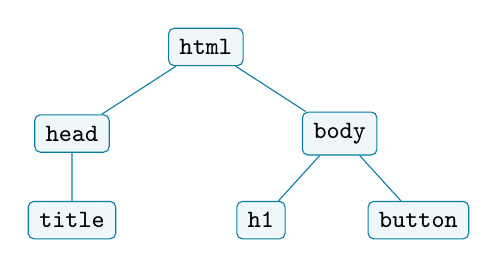
\begin{tikzpicture}[
  n/.style={draw=reactblue, rounded corners=2pt, fill=reactblue!6, font=\small\ttfamily, inner sep=4pt},
  level distance=1.1cm,
  level 1/.style={sibling distance=3.4cm},
  level 2/.style={sibling distance=2cm},
  edge from parent/.style={draw, reactblue}]
\node[n] {html}
  child {node[n] {head} child {node[n] {title}}}
  child {node[n] {body}
    child {node[n] {h1}}
    child {node[n] {button}}
  };
\end{tikzpicture}
\end{center}

Modificar el DOM a mano es posible, pero se vuelve difícil de mantener cuando la página crece. React resuelve eso.

\subsection{Imperativo y declarativo}

Compara un contador escrito con JavaScript puro y con React.

\textbf{JavaScript puro (imperativo).} Tú das cada instrucción para cambiar la pantalla:
\begin{lstlisting}[language=JSX]
let cuenta = 0
const boton = document.querySelector('#boton')
const texto = document.querySelector('#texto')

boton.addEventListener('click', () => {
  cuenta = cuenta + 1
  texto.textContent = `Clics: ${cuenta}` // tu actualizas el DOM
})
\end{lstlisting}

\textbf{React (declarativo).} Describes cómo debe verse la pantalla para cada valor de los datos, y React hace los cambios:
\begin{lstlisting}[language=JSX]
function Contador() {
  const [cuenta, setCuenta] = useState(0)
  return <button onClick={() => setCuenta(cuenta + 1)}>Clics: {cuenta}</button>
}
\end{lstlisting}

En el segundo caso no hay ninguna línea que modifique el DOM. Solo cambias el dato (\cmd{cuenta}) y la pantalla se ajusta. Esa es la idea central de React: \textbf{la interfaz es una función de los datos}.

\subsection{Qué es un componente}

Mira cualquier sitio web y divídelo en rectángulos: barra de navegación, tarjeta de producto, botón, pie de página. Cada rectángulo que tiene sentido por sí solo puede ser un componente. Un componente reúne en un mismo lugar la estructura (JSX), el aspecto (CSS) y el comportamiento (JavaScript) de esa parte, y se puede usar tantas veces como quieras.

%=====================================================
\section{El JavaScript que necesitas}\label{sec:js}

React es JavaScript. La mayoría de las dificultades al empezar vienen de sintaxis moderna del lenguaje y no de React. Esta sección repasa lo que vas a usar todo el tiempo.

\begin{nota}
Todos los ejemplos de esta sección están en \cmd{repaso-js/repaso.js} del proyecto de acompañamiento. Ejecútalos con \cmd{npm run repaso} y verás los resultados en la terminal. También puedes probar cada línea en la consola del navegador (\cmd{F12}).
\end{nota}

\subsection{\texttt{const} y \texttt{let}}

\begin{lstlisting}[language=JSX]
const curso = 'React' // no se puede reasignar
let inscritos = 30    // se puede reasignar
inscritos = inscritos + 5
\end{lstlisting}

Usa \cmd{const} por defecto y \cmd{let} solo cuando el valor deba cambiar. Evita \cmd{var}. En React casi todo es \cmd{const}, incluso el estado: \cmd{const [cuenta, setCuenta]}. El valor no se reasigna; React entrega uno nuevo en cada render.

\subsection{Template literals}

Texto entre comillas invertidas (\verb|`|) que permite insertar variables con \verb|${ }|:
\begin{lstlisting}[language=JSX]
console.log(`El curso ${curso} tiene ${inscritos} inscritos`)
\end{lstlisting}

En React se usan para armar clases CSS o URLs: \verb|className={`boton boton-${variante}`}|.

\subsection{Funciones flecha}

\begin{lstlisting}[language=JSX]
function sumarClasica(a, b) {
  return a + b
}
const sumar = (a, b) => a + b          // una expresion: retorno implicito
const doble = (n) => n * 2
const crearUsuario = (nombre) => ({ nombre, activo: true }) // objeto entre ()
\end{lstlisting}

Si el cuerpo es una sola expresión, se omiten las llaves y el \cmd{return}. Para devolver un objeto de forma implícita hay que envolverlo en paréntesis, porque las llaves solas se leerían como bloque. En React las verás en eventos (\cmd{onClick=\{() => ...\}}) y dentro de \cmd{map}.

\subsection{Desestructuración}

Extrae valores de objetos y arreglos en variables:
\begin{lstlisting}[language=JSX]
const alumno = { nombre: 'Pedro', edad: 22, carrera: 'Informatica' }
const { nombre, edad } = alumno
const { carrera: programa, sede = 'Vina del Mar' } = alumno // renombrar y por defecto

const colores = ['rojo', 'verde', 'azul']
const [primero, segundo] = colores
\end{lstlisting}

Con objetos importan los \textbf{nombres}; con arreglos importa la \textbf{posición}. Las props se reciben desestructurando un objeto (\cmd{function Tarjeta(\{ titulo \})}) y \cmd{useState} devuelve un arreglo de dos posiciones, por eso puedes llamarlas como quieras.

\subsection{Spread (\texttt{...})}

Copia el contenido de un arreglo u objeto dentro de otro nuevo:
\begin{lstlisting}[language=JSX]
const masColores = [...colores, 'negro']   // copia y agrega
const alumnoMayor = { ...alumno, edad: 23 } // copia y reemplaza edad
// alumno sigue teniendo edad 22
\end{lstlisting}

Es la herramienta principal para actualizar estado sin modificar el original.

\subsection{Métodos de arreglos}

Ninguno de estos métodos modifica el arreglo original.

\begin{lstlisting}[language=JSX]
const productos = [
  { id: 1, nombre: 'Teclado', precio: 25990, stock: 4 },
  { id: 2, nombre: 'Mouse', precio: 12990, stock: 0 },
  { id: 3, nombre: 'Monitor', precio: 149990, stock: 2 },
]
productos.map((p) => p.nombre)          // ['Teclado', 'Mouse', 'Monitor']
productos.filter((p) => p.stock > 0)    // Teclado y Monitor
productos.find((p) => p.id === 3)       // el objeto del Monitor
productos.some((p) => p.stock === 0)    // true
productos.reduce((total, p) => total + p.precio, 0) // 188970
\end{lstlisting}

\begin{center}
\small
\begin{tabular}{>{\ttfamily}l p{5.3cm} p{5.3cm}}
\toprule
\textrm{\textbf{Método}} & \textbf{Devuelve} & \textbf{Uso típico en React} \\
\midrule
map & Arreglo nuevo del mismo largo, transformado. & Convertir datos en elementos JSX. \\
filter & Arreglo nuevo solo con los que cumplen. & Buscar, eliminar un elemento del estado. \\
find & El primer elemento que cumple, o \cmd{undefined}. & Obtener el elemento seleccionado. \\
some & \cmd{true} o \cmd{false}. & Saber si mostrar un aviso. \\
reduce & Un solo valor acumulado. & Totales y sumas. \\
\bottomrule
\end{tabular}
\end{center}

\begin{atencion}
\cmd{sort}, \cmd{push}, \cmd{pop}, \cmd{splice} y \cmd{reverse} sí modifican el arreglo original. Con estado, aplícalos sobre una copia: \cmd{[...lista].sort()}.
\end{atencion}

\subsection{Condiciones cortas}

\begin{lstlisting}[language=JSX]
nota >= 4 ? 'Aprobado' : 'Reprobado'   // ternario: una cosa u otra
nota > 6 && 'Con distincion'           // && : el valor si se cumple, false si no
apodo ?? 'Sin apodo'                   // ?? : valor de reemplazo si es null o undefined
config.idioma?.codigo                  // ?. : undefined en vez de error si no existe
\end{lstlisting}

Dentro de JSX no se puede escribir un \cmd{if}, así que estas formas son las que se usan en el \cmd{return}. El \cmd{?.} es muy útil con datos que llegan de una API y todavía no están cargados.

\subsection{Módulos: \texttt{import} y \texttt{export}}

\begin{lstlisting}[language=JSX,title={\small\ttfamily repaso-js/utilidades.js}]
export const IVA = 0.19                       // exportacion nombrada
export function conIva(precio) { return Math.round(precio * (1 + IVA)) }
export default function formatearPesos(valor) { // exportacion por defecto
  return '$' + valor.toLocaleString('es-CL')
}
\end{lstlisting}
\begin{lstlisting}[language=JSX]
import formatearPesos, { IVA, conIva } from './utilidades.js'
\end{lstlisting}

Un archivo tiene como máximo un \cmd{export default}, que se importa sin llaves y con el nombre que quieras. Las exportaciones nombradas se importan entre llaves con su nombre exacto. Por eso \cmd{import \{ useState \} from 'react'} lleva llaves.

\subsection{Promesas y \texttt{async}/\texttt{await}}

Algunas operaciones tardan, como pedir datos a un servidor. Una \textbf{promesa} representa un resultado que llegará después. \cmd{await} espera ese resultado sin bloquear la página, y solo se puede usar dentro de una función \cmd{async}:
\begin{lstlisting}[language=JSX]
async function cargarUsuarios() {
  try {
    const res = await fetch('https://jsonplaceholder.typicode.com/users')
    const datos = await res.json()
    console.log(datos)
  } catch (error) {
    console.log('Algo fallo:', error.message)
  }
}
\end{lstlisting}

Es otra forma de escribir las cadenas \cmd{.then().catch()}. Las dos hacen lo mismo; \cmd{async}/\cmd{await} suele leerse mejor.

\begin{ejercicio}[de JavaScript]
Con el arreglo \cmd{productos}, obtén en una sola línea los nombres de los productos con stock, en mayúsculas. Luego calcula el valor total del inventario (precio por stock de cada producto).
\end{ejercicio}


%=====================================================
\section{Instalación de Node.js}

Instala siempre la versión \textbf{LTS} (\emph{Long Term Support}), que es la versión estable recomendada para trabajar. Vite exige Node.js 20.19 o superior (o 22.12 en adelante), así que cualquier LTS vigente sirve.

\subsection{Windows}

\textbf{Opción A: instalador oficial.}
\begin{enumerate}[leftmargin=*]
  \item Entra a \url{https://nodejs.org} y descarga el instalador LTS (\cmd{.msi}).
  \item Ejecútalo y acepta las opciones por defecto. Deja marcada la casilla que agrega Node al \cmd{PATH}.
  \item Cierra y vuelve a abrir la terminal (PowerShell o CMD) para que reconozca los comandos nuevos.
\end{enumerate}

\textbf{Opción B: desde la terminal con winget.}
\begin{terminal}
winget install OpenJS.NodeJS.LTS
\end{terminal}

\subsection{macOS}

Puedes usar el instalador \cmd{.pkg} de \url{https://nodejs.org} o Homebrew:
\begin{terminal}
brew install node
\end{terminal}

\subsection{Linux (Ubuntu / Debian)}

Los repositorios de la distribución suelen traer versiones antiguas. Lo más limpio es usar \textbf{nvm} (ver sección \ref{sec:nvm}).

\subsection{Opción recomendada: nvm}\label{sec:nvm}

\textbf{nvm} (\emph{Node Version Manager}) permite tener varias versiones de Node y cambiar entre ellas. Es útil cuando un proyecto antiguo pide otra versión.

En macOS y Linux:
\begin{terminal}
curl -o- https://raw.githubusercontent.com/nvm-sh/nvm/master/install.sh | bash
# cierra y abre la terminal
nvm install --lts
nvm use --lts
\end{terminal}

En Windows se usa un proyecto distinto, \textbf{nvm-windows} (\url{https://github.com/coreybutler/nvm-windows}). Tras instalarlo:
\begin{terminal}
nvm install lts
nvm use lts
\end{terminal}

\subsection{Verificar la instalación}

\begin{terminal}
node -v
npm -v
\end{terminal}

Ambos comandos deben responder con un número de versión, por ejemplo \cmd{v22.x.x} y \cmd{10.x.x}.

\begin{atencion}
Si aparece ``\emph{node no se reconoce como un comando}'', cierra todas las terminales (y VS Code) y ábrelas de nuevo. Si el problema sigue, reinicia el equipo o revisa que la carpeta de Node esté en la variable \cmd{PATH}.
\end{atencion}

\begin{atencion}
En Windows, PowerShell puede bloquear \cmd{npm} con un error de \emph{ejecución de scripts deshabilitada}. Abre PowerShell y ejecuta:
\cmd{Set-ExecutionPolicy -Scope CurrentUser RemoteSigned}
\end{atencion}

%=====================================================
\section{Preparar el editor}

\begin{enumerate}[leftmargin=*]
  \item Descarga Visual Studio Code desde \url{https://code.visualstudio.com}.
  \item Instala estas extensiones desde el panel de extensiones (\cmd{Ctrl+Shift+X}):
  \begin{itemize}
    \item \textbf{ES7+ React/Redux/React-Native snippets}: atajos como \cmd{rafce} que generan un componente completo.
    \item \textbf{Oxc}: muestra en el editor los avisos de oxlint, el revisor de código que trae la plantilla de Vite.
    \item \textbf{Prettier}: formatea el código al guardar.
  \end{itemize}
  \item En el navegador (Chrome o Firefox) instala \textbf{React Developer Tools}. Agrega las pestañas \emph{Components} y \emph{Profiler} a las herramientas de desarrollo para inspeccionar componentes, props y estado.
\end{enumerate}

%=====================================================
\section{Crear el primer proyecto con Vite}

\begin{nota}
Durante años se usó \cmd{create-react-app}. Hoy está descontinuado y la documentación oficial de React ya no lo recomienda. Para aprender, Vite es la opción más simple y rápida.
\end{nota}

\subsection{Generar el proyecto}

Abre una terminal en la carpeta donde guardas tus proyectos y ejecuta:
\begin{terminal}
npm create vite@latest mi-primera-app
\end{terminal}

El asistente hará dos preguntas. Responde así:
\begin{itemize}
  \item \textbf{Select a framework:} \cmd{React}
  \item \textbf{Select a variant:} \cmd{JavaScript} (más adelante puedes probar \cmd{TypeScript})
\end{itemize}

También puedes indicar la plantilla directamente y saltarte las preguntas:
\begin{terminal}
npm create vite@latest mi-primera-app -- --template react
\end{terminal}

\subsection{Instalar dependencias y ejecutar}

\begin{terminal}
cd mi-primera-app
npm install
npm run dev
\end{terminal}

La terminal mostrará una dirección como \cmd{http://localhost:5173}. Ábrela en el navegador y verás la página de ejemplo con un contador.

\begin{nota}
El servidor de desarrollo tiene \emph{recarga en caliente} (HMR): cada vez que guardas un archivo, el navegador se actualiza solo. Para detener el servidor presiona \cmd{Ctrl+C} en la terminal.
\end{nota}

Para abrir el proyecto en VS Code desde la terminal:
\begin{terminal}
code .
\end{terminal}

\subsection{Proyecto de acompañamiento}

Junto a esta guía se entrega \cmd{guia-react.zip}, con todos los ejemplos funcionando. Cada pestaña de la aplicación corresponde a un capítulo y cada ejemplo muestra la ruta del archivo que lo contiene, para que puedas abrirlo, modificarlo y ver el cambio al instante. Para usarlo:
\begin{terminal}
# descomprime el zip y entra a la carpeta
cd guia-react
npm install        # la carpeta node_modules no viene en el zip
npm run dev
\end{terminal}

\begin{lstlisting}[language={},numbers=none]
karma.conf.cjs                configuracion de las pruebas
repaso-js/                    repaso de JavaScript (npm run repaso)
docs/                         esta guia en PDF y LaTeX
src/
|-- main.jsx                  punto de entrada comentado
|-- App.jsx                   navegacion entre secciones
|-- index.css                 variables y reglas base
|-- styles/utilidades.css     clases compartidas
|-- logica/                   funciones puras y sus archivos .spec.js
`-- components/
    |-- Ejemplo.jsx           marco con titulo y archivo de cada ejemplo
    |-- basicos/              ejemplos principales de cada capitulo
    |                         cada componente con estilos trae su .css al lado
    |-- jsx/ props/ estado/ eventos/ condicional/
    |-- listas/ formularios/ efectos/   ejemplos adicionales
    |-- render/DemoRender.jsx experimento de renderizado
    `-- tareas/               proyecto integrador
\end{lstlisting}

%=====================================================
\section{Estructura del proyecto}

\begin{lstlisting}[language={},numbers=none]
mi-primera-app/
|-- node_modules/      dependencias instaladas (no se edita ni se sube a Git)
|-- public/            archivos estaticos servidos tal cual
|-- src/
|   |-- assets/        imagenes y recursos importados desde el codigo
|   |-- App.css
|   |-- App.jsx        componente principal
|   |-- index.css      estilos globales
|   `-- main.jsx       punto de entrada: monta React en la pagina
|-- index.html         unica pagina HTML; contiene <div id="root">
|-- package.json       nombre, scripts y dependencias
|-- vite.config.js     configuracion de Vite
`-- .oxlintrc.json     reglas de oxlint (revisor de codigo)
\end{lstlisting}

El recorrido completo desde \cmd{index.html} hasta tu componente se explica en la sección \ref{sec:arranque}.

\subsection{Los scripts de \texttt{package.json}}

\begin{center}
\begin{tabular}{>{\ttfamily}l p{9.5cm}}
\toprule
\textrm{\textbf{Comando}} & \textbf{Qué hace} \\
\midrule
npm run dev & Levanta el servidor de desarrollo. \\
npm run build & Genera la versión optimizada para producción en la carpeta \cmd{dist/}. \\
npm run preview & Sirve localmente el contenido de \cmd{dist/} para probarlo. \\
npm run lint & Revisa el código con oxlint. \\
npm test & Ejecuta las pruebas unitarias con Karma y Jasmine. \\
npm run repaso & Corre el repaso de JavaScript en la terminal. \\
\bottomrule
\end{tabular}
\end{center}

\subsection{Dejar el proyecto limpio}

Antes de escribir tu propio código, reemplaza el contenido de \cmd{src/App.jsx} por:
\begin{lstlisting}[language=JSX,title={\small\ttfamily src/App.jsx}]
function App() {
  return (
    <main>
      <h1>Hola, React</h1>
      <p>Mi primera aplicacion.</p>
    </main>
  )
}

export default App
\end{lstlisting}

Borra también el contenido de \cmd{src/App.css} y \cmd{src/index.css} para partir sin estilos heredados.

%=====================================================
\section{Cómo arranca la aplicación: los componentes del render}\label{sec:arranque}

Entre abrir \cmd{localhost:5173} y ver tu componente en pantalla intervienen varias piezas. Conocerlas ayuda a entender los errores de arranque y qué hace cada línea de \cmd{main.jsx}.

\begin{center}
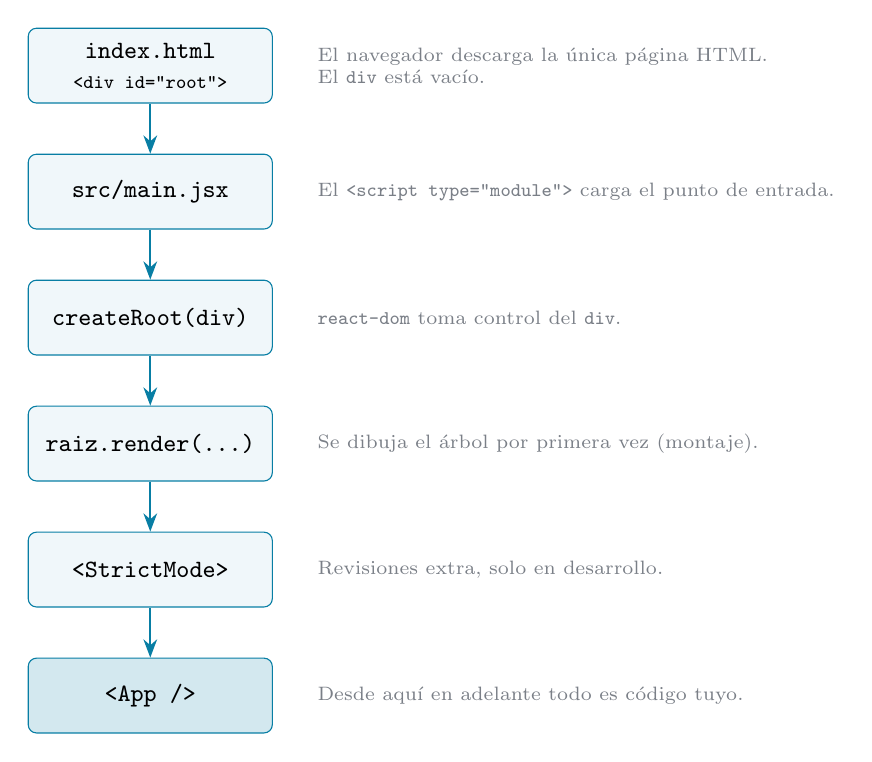
\begin{tikzpicture}[
  caja/.style={draw=reactblue, rounded corners=3pt, fill=reactblue!6, minimum width=3.1cm,
               minimum height=0.95cm, align=center, font=\small},
  obs/.style={font=\scriptsize\color{com}, align=left, anchor=west},
  flecha/.style={-{Stealth}, thick, reactblue}]
\node[caja] (html) at (0,0) {\texttt{index.html}\\\scriptsize\texttt{<div id="root">}};
\node[caja] (main) at (0,-1.6) {\texttt{src/main.jsx}};
\node[caja] (root) at (0,-3.2) {\texttt{createRoot(div)}};
\node[caja] (rend) at (0,-4.8) {\texttt{raiz.render(...)}};
\node[caja] (sm)   at (0,-6.4) {\texttt{<StrictMode>}};
\node[caja, fill=reactblue!18] (app) at (0,-8.0) {\texttt{<App />}};
\foreach \a/\b in {html/main, main/root, root/rend, rend/sm, sm/app}
  \draw[flecha] (\a) -- (\b);
\node[obs] at (2,0)    {El navegador descarga la única página HTML.\\El \texttt{div} está vacío.};
\node[obs] at (2,-1.6) {El \texttt{<script type="module">} carga el punto de entrada.};
\node[obs] at (2,-3.2) {\texttt{react-dom} toma control del \texttt{div}.};
\node[obs] at (2,-4.8) {Se dibuja el árbol por primera vez (montaje).};
\node[obs] at (2,-6.4) {Revisiones extra, solo en desarrollo.};
\node[obs] at (2,-8.0) {Desde aquí en adelante todo es código tuyo.};
\end{tikzpicture}
\end{center}

\subsection{\texttt{index.html} y el \texttt{div} raíz}

Es la única página HTML de la aplicación. Su \cmd{body} contiene dos líneas:
\begin{lstlisting}[language=HTML,numbers=none]
<div id="root"></div>
<script type="module" src="/src/main.jsx"></script>
\end{lstlisting}

Si abres ``ver código fuente'' en el navegador verás ese \cmd{div} vacío. Todo el contenido lo inserta JavaScript después. Por eso a este tipo de aplicación se le llama \emph{SPA} (\emph{Single Page Application}): hay una sola página y React cambia su contenido.

\subsection{\texttt{main.jsx}, línea por línea}

\begin{lstlisting}[language=JSX,title={\small\ttfamily src/main.jsx}]
import { StrictMode } from 'react'
import { createRoot } from 'react-dom/client'
import './index.css'
import App from './App.jsx'

const contenedor = document.getElementById('root')
const raiz = createRoot(contenedor)

raiz.render(
  <StrictMode>
    <App />
  </StrictMode>,
)
\end{lstlisting}

La plantilla de Vite escribe las líneas 6 a 9 en una sola expresión encadenada. Aquí están separadas para ver cada paso.

\begin{description}[leftmargin=0pt, style=nextline, itemsep=0.5em]
\item[Líneas 1 y 2: dos paquetes distintos.]
\cmd{react} define qué es un componente, JSX y los hooks. \cmd{react-dom} sabe traducir eso a elementos del navegador (el DOM). Esta separación existe porque React también dibuja en otros destinos: React Native usa el mismo \cmd{react} con otro paquete de dibujo.

\item[Línea 3: \texttt{import './index.css'}.]
Importar un CSS desde JavaScript no es estándar del lenguaje. Vite lo intercepta e inyecta los estilos en la página. Los estilos quedan globales.

\item[Línea 4: \texttt{import App}.]
Trae el componente raíz de tu aplicación.

\item[Línea 6: \texttt{document.getElementById('root')}.]
Es DOM puro, no React. Busca el \cmd{div} de \cmd{index.html}. Si cambias el id en un archivo y no en el otro, aparece el error \emph{Target container is not a DOM element}.

\item[Línea 7: \texttt{createRoot(contenedor)}.]
Crea una \textbf{raíz de React} sobre ese \cmd{div}. A partir de este momento React administra todo lo que ocurre dentro de él, y no debes modificar ese contenido con \cmd{innerHTML} u otros métodos del DOM. Se llama una sola vez en toda la aplicación.

\item[Línea 9: \texttt{raiz.render(...)}.]
Recibe un elemento JSX y lo dibuja por primera vez. A este primer dibujo se le llama \textbf{montaje}. Después no vuelves a llamar a \cmd{render}: las actualizaciones posteriores las disparan los cambios de estado dentro de los componentes.

\item[Línea 10: \texttt{<StrictMode>}.]
Es un componente que no produce nada visible. Solo actúa en desarrollo y desaparece en \cmd{npm run build}. Hace dos cosas: ejecuta cada componente dos veces para detectar código impuro, y monta, desmonta y vuelve a montar los efectos para revelar limpiezas olvidadas. Por eso ves \cmd{console.log} duplicados o dos peticiones \cmd{fetch} en la pestaña Red.

\item[Línea 11: \texttt{<App />}.]
Es la raíz de tu árbol de componentes. Todo lo que construyas cuelga de aquí.
\end{description}

\subsection{El árbol de componentes}

Cada componente puede usar otros dentro de su JSX, así que la aplicación forma un árbol. Este es el del proyecto de acompañamiento cuando está activa la pestaña de tareas:

\begin{center}
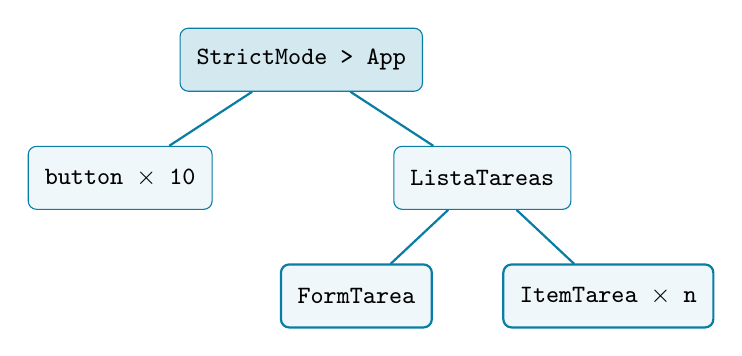
\begin{tikzpicture}[
  n/.style={draw=reactblue, rounded corners=3pt, fill=reactblue!6, font=\small\ttfamily,
            minimum height=0.8cm, inner xsep=6pt},
  level distance=1.5cm,
  level 1/.style={sibling distance=4.6cm},
  level 2/.style={sibling distance=3.2cm},
  edge from parent/.style={draw, reactblue, thick}]
\node[n, fill=reactblue!18] {StrictMode > App}
  child {node[n] {button $\times$ 10}}
  child {node[n] {ListaTareas}
    child {node[n] {FormTarea}}
    child {node[n] {ItemTarea $\times$ n}}
  };
\end{tikzpicture}
\end{center}

Los datos bajan por el árbol mediante props (de \cmd{ListaTareas} a \cmd{ItemTarea}). Los avisos suben mediante funciones recibidas como props (\cmd{onEliminar}, \cmd{onAgregar}).

\subsection{Las tres fases de cada render}

En React, \textbf{renderizar} significa llamar a la función del componente para obtener su JSX. Que un componente se renderice no implica que la pantalla cambie. Cada actualización pasa por tres fases:

\begin{center}
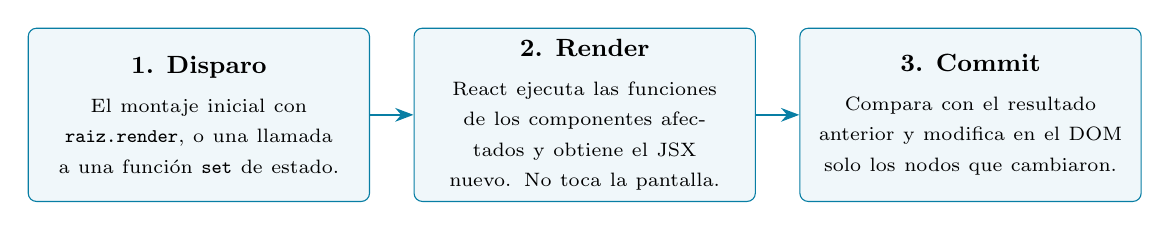
\begin{tikzpicture}[
  f/.style={draw=reactblue, rounded corners=3pt, fill=reactblue!6, text width=4.1cm,
            align=center, font=\small, minimum height=2.2cm},
  flecha/.style={-{Stealth}, thick, reactblue}]
\node[f] (t) at (0,0) {\textbf{1. Disparo}\\[3pt]\scriptsize El montaje inicial con \texttt{raiz.render}, o una llamada a una función \texttt{set} de estado.};
\node[f] (r) at (4.9,0) {\textbf{2. Render}\\[3pt]\scriptsize React ejecuta las funciones de los componentes afectados y obtiene el JSX nuevo. No toca la pantalla.};
\node[f] (c) at (9.8,0) {\textbf{3. Commit}\\[3pt]\scriptsize Compara con el resultado anterior y modifica en el DOM solo los nodos que cambiaron.};
\draw[flecha] (t) -- (r);
\draw[flecha] (r) -- (c);
\end{tikzpicture}
\end{center}

Una forma de verlo: la fase de render dibuja un plano nuevo de la casa y la fase de commit ejecuta en obra solo las diferencias con el plano anterior. Si nada cambió, la obra no se toca.

Esta es la razón por la que la función de un componente debe ser \textbf{pura}: con las mismas props y el mismo estado debe devolver el mismo JSX, sin modificar variables externas, sin hacer peticiones y sin tocar el DOM. Lo que tenga efectos externos va en manejadores de eventos o en \cmd{useEffect}.

\begin{nota}
En la sección \ref{sec:rerender} se explica qué provoca que un componente se vuelva a renderizar, una vez que conozcas el estado.
\end{nota}

%=====================================================
\section{JSX: HTML dentro de JavaScript}\label{sec:jsx}

JSX es una sintaxis que permite escribir estructuras parecidas a HTML dentro de JavaScript. Vite la traduce a llamadas de JavaScript normales.

\subsection{Reglas básicas}

\begin{enumerate}[leftmargin=*]
  \item \textbf{Un solo elemento raíz.} Si necesitas devolver varios elementos, envuélvelos en un \cmd{div} o en un fragmento vacío \cmd{<>...</>}.
  \item \textbf{Todas las etiquetas se cierran}, incluso las que en HTML no lo requieren: \cmd{<img />}, \cmd{<br />}, \cmd{<input />}.
  \item \textbf{Atributos en camelCase}: \cmd{class} pasa a ser \cmd{className}, \cmd{for} pasa a ser \cmd{htmlFor}, \cmd{onclick} pasa a ser \cmd{onClick}.
  \item \textbf{Las llaves \cmd{\{ \}} insertan JavaScript}: variables, operaciones o llamadas a funciones.
\end{enumerate}

\begin{lstlisting}[language=JSX]
function Perfil() {
  const nombre = 'Ana'
  const edad = 21
  const foto = 'https://i.pravatar.cc/100'

  return (
    <>
      <img src={foto} alt={nombre} className="avatar" />
      <h2>{nombre.toUpperCase()}</h2>
      <p>El proximo anio tendra {edad + 1} anios.</p>
    </>
  )
}
\end{lstlisting}

\subsection{Estilos}

La forma habitual es escribir CSS normal en un archivo e importarlo desde el componente:
\begin{lstlisting}[language=JSX]
import './Perfil.css'
// ...
<div className="tarjeta">...</div>
\end{lstlisting}

También se pueden poner estilos en línea con el atributo \cmd{style}, que recibe un \textbf{objeto} con las propiedades en camelCase. Por eso aparecen dobles llaves: las externas abren JavaScript y las internas son las del objeto.
\begin{lstlisting}[language=JSX]
<p style={{ color: 'white', backgroundColor: '#087EA4', padding: 8 }}>
  Texto destacado
</p>
\end{lstlisting}

La sección \ref{sec:css} trata el tema completo: dónde poner cada archivo, variables CSS, CSS Modules y clases dinámicas.

\subsection{Qué se puede poner entre llaves}

Entre llaves va cualquier \textbf{expresión}: algo que produce un valor. Variables, operaciones, llamadas a funciones, ternarios y \cmd{map} son expresiones. Las \textbf{sentencias} como \cmd{if}, \cmd{for} o \cmd{const x = 1} no lo son y no se pueden escribir dentro del JSX. Se escriben antes del \cmd{return}.

\begin{center}
\small
\begin{tabular}{p{6.3cm} p{6.3cm}}
\toprule
\textbf{Válido} & \textbf{No válido} \\
\midrule
\cmd{\{nombre\}} & \cmd{\{if (activo) \{ ... \}\}} \\
\cmd{\{precio * 1.19\}} & \cmd{\{for (let i = 0; ...)\}} \\
\cmd{\{activo ? 'Sí' : 'No'\}} & \cmd{\{const x = 5\}} \\
\cmd{\{lista.map(...)\}} & \cmd{\{alumno\}} si es un objeto \\
\bottomrule
\end{tabular}
\end{center}

Un objeto no se puede mostrar directamente: React no sabe cómo convertirlo en texto y lanza el error \emph{Objects are not valid as a React child}. Muestra sus propiedades (\cmd{\{alumno.nombre\}}) o conviértelo con \cmd{JSON.stringify}. Los valores \cmd{true}, \cmd{false}, \cmd{null} y \cmd{undefined} no muestran nada.

\subsection{Más ejemplos}

\textbf{Datos, cálculos y JSX en variables.} Antes del \cmd{return} puedes hacer cualquier cálculo. Aquí se obtienen las iniciales con métodos de texto y arreglos, y se guarda un fragmento de JSX en una variable para usarlo después.

\begin{lstlisting}[language=JSX,title={\small\ttfamily src/components/jsx/TarjetaPresentacion.jsx}]
// Datos fuera del componente: no cambian, así que no necesitan estado.
const persona = {
  nombre: 'Valentina Rojas',
  carrera: 'Ingeniería en Informática',
  semestre: 2,
  intereses: ['React', 'Bases de datos', 'Diseño'],
}

function TarjetaPresentacion() {
  // Cálculos normales de JavaScript antes del return
  const iniciales = persona.nombre
    .split(' ')
    .map((palabra) => palabra[0])
    .join('')
  const esPrimerAnio = persona.semestre <= 2

  // Una variable también puede guardar JSX
  const etiqueta = esPrimerAnio ? <span className="badge">Primer año</span> : null

  return (
    <div className="caja">
      {/* Así se escribe un comentario dentro de JSX */}
      <div className="avatar-texto">{iniciales}</div>
      <h3>
        {persona.nombre} {etiqueta}
      </h3>
      <p>
        {persona.carrera}, semestre {persona.semestre}
      </p>
      <p>Intereses: {persona.intereses.join(', ')}</p>
      <p>Cantidad de intereses: {persona.intereses.length}</p>
    </div>
  )
}

export default TarjetaPresentacion
\end{lstlisting}

Observa que \cmd{persona} está fuera de la función. Los datos que no cambian no necesitan estado ni tienen que redefinirse en cada render.

%=====================================================
\section{Componentes}

Un componente es una función cuyo nombre empieza con \textbf{mayúscula} y que devuelve JSX. La mayúscula es obligatoria: así React distingue \cmd{<Boton />} (tu componente) de \cmd{<button>} (etiqueta HTML).

Crea la carpeta \cmd{src/components} y dentro el archivo \cmd{Saludo.jsx}:
\begin{lstlisting}[language=JSX,title={\small\ttfamily src/components/Saludo.jsx}]
function Saludo() {
  return <h2>Bienvenido al curso</h2>
}

export default Saludo
\end{lstlisting}

Úsalo en \cmd{App.jsx}:
\begin{lstlisting}[language=JSX,title={\small\ttfamily src/App.jsx}]
import Saludo from './components/Saludo'

function App() {
  return (
    <main>
      <h1>Hola, React</h1>
      <Saludo />
      <Saludo />
    </main>
  )
}

export default App
\end{lstlisting}

\begin{nota}
Con la extensión de snippets instalada, escribe \cmd{rafce} en un archivo vacío y presiona \cmd{Tab}. Se genera el esqueleto del componente con el nombre del archivo.
\end{nota}

\subsection{Más ejemplos}

\textbf{Composición.} Construir una interfaz consiste en combinar componentes pequeños. Este archivo define tres componentes y exporta dos de ellos por nombre, además del componente por defecto.

\begin{lstlisting}[language=JSX,title={\small\ttfamily src/components/jsx/Composicion.jsx}]
// Un archivo puede tener varios componentes.
// "export" sin default permite importarlos por nombre: import { Encabezado } from './Composicion'

export function Encabezado({ titulo }) {
  return (
    <header className="encabezado">
      <strong>{titulo}</strong>
    </header>
  )
}

export function PiePagina() {
  const anio = new Date().getFullYear()
  return <footer className="pie">© {anio} Mi sitio</footer>
}

// Layout arma la estructura y deja un espacio (children) para el contenido.
function Layout({ titulo, children }) {
  return (
    <div className="layout">
      <Encabezado titulo={titulo} />
      <div className="contenido">{children}</div>
      <PiePagina />
    </div>
  )
}

function Composicion() {
  return (
    <Layout titulo="Mi tienda">
      <p>Este contenido lo decide quien usa Layout.</p>
      <p>El encabezado y el pie se repiten sin volver a escribirlos.</p>
    </Layout>
  )
}

export default Composicion
\end{lstlisting}

\cmd{Layout} no sabe qué contenido va a mostrar: lo recibe en \cmd{children}. Así puedes tener una misma estructura de página con contenidos distintos. Desde otro archivo se importaría así:
\begin{lstlisting}[language=JSX]
import Composicion, { Encabezado, PiePagina } from './components/jsx/Composicion'
\end{lstlisting}

\subsection{Cómo dividir en componentes}

Algunas pistas para decidir cuándo crear un componente nuevo:
\begin{itemize}
  \item Una parte de la interfaz se repite (tarjetas, filas de una tabla, botones con el mismo estilo).
  \item Un componente supera las 80 o 100 líneas y cuesta leerlo.
  \item Una parte tiene su propio estado que al resto no le interesa.
\end{itemize}
Un archivo por componente es la convención más común. El nombre del archivo coincide con el del componente.

%=====================================================
\section{Estilos: CSS en React}\label{sec:css}

React no trae su propio sistema de estilos: se usa CSS normal. Lo que cambia es \textbf{dónde} vive ese CSS y \textbf{cómo} llega a la página.

\subsection{Cuatro formas de aplicar estilos}

\begin{center}
\small
\begin{tabular}{p{3.1cm} p{4.6cm} p{5.6cm}}
\toprule
\textbf{Forma} & \textbf{Cómo se escribe} & \textbf{Cuándo conviene} \\
\midrule
CSS global & Un archivo importado en \cmd{main.jsx}. & Variables, reglas base y clases compartidas. \\
\addlinespace
CSS por componente & Un \cmd{.css} junto al \cmd{.jsx}, importado por él. & Lo más común. Mantiene cerca el componente y su estilo. \\
\addlinespace
CSS Modules & Archivo \cmd{.module.css} importado como objeto. & Cuando quieres nombres de clase que no puedan chocar. \\
\addlinespace
Estilos en línea & Atributo \cmd{style} con un objeto. & Valores calculados en tiempo de ejecución. \\
\bottomrule
\end{tabular}
\end{center}

Además existen herramientas externas como Tailwind CSS, que usa clases utilitarias, o styled-components, que escribe el CSS dentro del JavaScript. No las necesitas para empezar.

\subsection{Un detalle importante: el CSS importado es global}

Cuando escribes \cmd{import './Boton.css'} dentro de \cmd{Boton.jsx}, Vite inserta ese archivo en la página completa. El import sirve para \textbf{organizar} el proyecto y para que Vite sepa qué incluir, pero la clase \cmd{.boton} queda disponible en toda la aplicación. Si otro archivo define también \cmd{.boton}, la última regla cargada gana.

Dos maneras de evitar choques de nombres:
\begin{enumerate}[leftmargin=*]
  \item \textbf{Prefijar las clases} con el nombre del componente: \cmd{.tarjeta}, \cmd{.tarjeta-titulo}, \cmd{.tarjeta-precio}. Es la convención más usada y no requiere nada especial.
  \item \textbf{CSS Modules}, donde el navegador nunca ve tus nombres originales.
\end{enumerate}

\subsection{CSS global: variables y reglas base}

Las \textbf{variables CSS} se definen una vez en \cmd{:root} y se usan en todos los archivos con \cmd{var(--nombre)}. Cambiar un color del tema pasa a ser editar una línea.

\begin{lstlisting}[language=JSX,title={\small\ttfamily src/index.css}]
/* Estilos globales: se cargan una vez desde main.jsx y valen para toda la app. */

/* Variables CSS: se definen una vez y se reutilizan en todos los archivos */
:root {
  --color-principal: #087ea4;
  --color-principal-suave: #e6f4f9;
  --color-texto: #23272f;
  --color-tenue: #7a7f87;
  --color-borde: #e3e6ea;
  --color-fondo: #f6f7f9;
  --color-alerta: #b45309;
  --color-ok: #15803d;
  --color-peligro: #c0306f;
  --radio: 8px;
  --espacio: 12px;

  font-family: system-ui, -apple-system, 'Segoe UI', Roboto, sans-serif;
  color: var(--color-texto);
  background: var(--color-fondo);
}

* {
  box-sizing: border-box;
}

body {
  margin: 0;
}

/* Estilos base de los elementos del formulario, iguales en toda la app */
button {
  font: inherit;
  padding: 6px 12px;
  margin: 4px 4px 4px 0;
  border: 1px solid var(--color-principal);
  border-radius: 6px;
  background: white;
  color: var(--color-principal);
  cursor: pointer;
}

button:hover {
  background: var(--color-principal-suave);
}

button:disabled {
  opacity: 0.45;
  cursor: not-allowed;
}

input,
select,
textarea {
  font: inherit;
  padding: 6px 8px;
  border: 1px solid #c5cad3;
  border-radius: 6px;
}

pre {
  overflow-x: auto;
}
\end{lstlisting}

Las clases que varios componentes comparten viven aparte:

\begin{lstlisting}[language=JSX,title={\small\ttfamily src/styles/utilidades.css}]
/* Clases de uso general, compartidas por varios componentes. */

.caja {
  background: white;
  border: 1px solid var(--color-borde);
  border-radius: var(--radio);
  padding: var(--espacio) 16px;
  margin: 10px 0;
}

.fila {
  display: flex;
  gap: var(--espacio);
  flex-wrap: wrap;
  align-items: center;
}

.formulario {
  display: flex;
  flex-direction: column;
  gap: 6px;
  max-width: 380px;
}

.alerta {
  color: var(--color-alerta);
  font-weight: 600;
}

.ok {
  color: var(--color-ok);
  font-weight: 600;
}

.badge {
  background: var(--color-peligro);
  color: white;
  border-radius: 12px;
  padding: 2px 10px;
  font-size: 0.85rem;
}
\end{lstlisting}

Ambos archivos se cargan una sola vez, en el punto de entrada:
\begin{lstlisting}[language=JSX]
import './index.css'
import './styles/utilidades.css'
\end{lstlisting}

\subsection{CSS por componente}

Cada componente con estilos propios tiene un archivo con su mismo nombre, en la misma carpeta, y lo importa en la primera línea.

\begin{lstlisting}[language=JSX,title={\small\ttfamily src/components/props/Boton.css}]
/* Clase base más una clase por variante: boton-primario, boton-peligro... */
.boton {
  transition: background 0.15s;
}

.boton-primario {
  background: var(--color-principal);
  color: white;
}

.boton-primario:hover {
  background: #066880;
}

.boton-peligro {
  border-color: var(--color-peligro);
  color: var(--color-peligro);
}

.boton-peligro:hover {
  background: #fce7f0;
}
\end{lstlisting}
\begin{lstlisting}[language=JSX,title={\small\ttfamily src/components/props/Boton.jsx}]
import './Boton.css'

function Boton({ texto, variante = 'normal', deshabilitado = false, onClick }) {
  return (
    <button className={`boton boton-${variante}`} ...>{texto}</button>
  )
}
\end{lstlisting}

El patrón de una clase base más una clase por variante (\cmd{boton boton-primario}) es habitual: la base define lo común y la variante solo lo que cambia.

\subsection{CSS Modules}

Un archivo que termina en \cmd{.module.css} se importa como un objeto. Cada propiedad de ese objeto es el nombre real que tendrá la clase en el navegador, generado por Vite.

\begin{lstlisting}[language=JSX,title={\small\ttfamily src/components/listas/Buscador.module.css}]
/* CSS Module: Vite renombra estas clases al compilar (buscador -> _buscador_1a2b3)
   para que no choquen con clases de otros archivos. */
.controles {
  display: flex;
  gap: var(--espacio);
  flex-wrap: wrap;
}

.resumen {
  color: var(--color-tenue);
  font-size: 0.9rem;
}

.lista {
  list-style: none;
  padding: 0;
  margin: 0;
}

.lista li {
  padding: 6px 0;
  border-bottom: 1px solid var(--color-borde);
}

.vacio {
  color: var(--color-alerta);
  font-weight: 600;
}
\end{lstlisting}
\begin{lstlisting}[language=JSX]
import estilos from './Buscador.module.css'
// ...
<div className={estilos.controles}>
<p className={estilos.resumen}>...</p>
\end{lstlisting}

En pantalla, \cmd{controles} se convierte en algo como \cmd{\_controles\_18kl5\_3}. Como ese nombre es único, dos componentes pueden tener una clase \cmd{lista} sin interferirse. El costo es escribir \cmd{estilos.} en cada clase.

\begin{nota}
Los nombres con guion, como \cmd{.mi-clase}, se leen con corchetes: \cmd{estilos['mi-clase']}. Para evitarlo, en los CSS Modules se suele escribir en una sola palabra o en camelCase.
\end{nota}

\subsection{Clases dinámicas}

\cmd{className} recibe un texto, así que se arma con las mismas herramientas de JavaScript de siempre:
\begin{lstlisting}[language=JSX]
// Ternario: una clase u otra
<p className={aprobado ? 'ok' : 'alerta'}>{mensaje}</p>

// Clase fija mas una condicional
<div className={encima ? 'zona zona-activa' : 'zona'}>...</div>

// Template literal con un valor variable
<button className={`boton boton-${variante}`}>...</button>

// Varias condiciones: arreglo, filtrado y unido por espacios
<li className={['item', hecha && 'item-hecha', urgente && 'item-urgente']
  .filter(Boolean).join(' ')}>
\end{lstlisting}

El \cmd{.filter(Boolean)} descarta los \cmd{false} antes de unir, para que no queden espacios sobrantes.

\subsection{Estilos en línea}

El atributo \cmd{style} recibe un \textbf{objeto}, no un texto. Las propiedades van en camelCase y los valores como texto, salvo los números en píxeles:
\begin{lstlisting}[language=JSX]
<p style={{ color: 'white', backgroundColor: '#087EA4', padding: 8 }}>Destacado</p>

// Util cuando el valor se calcula
<div className="barra" style={{ width: `${porcentaje}%` }} />
\end{lstlisting}

Las dobles llaves confunden al principio: las externas abren JavaScript dentro de JSX y las internas son las del objeto. Úsalos solo para valores que cambian en tiempo de ejecución; el resto va en CSS, donde puedes usar \cmd{:hover}, \cmd{@media} y animaciones, cosa que los estilos en línea no permiten.

\subsection{Cómo quedan los archivos}

\begin{lstlisting}[language={},numbers=none]
src/
|-- index.css                         variables y reglas base
|-- styles/utilidades.css             clases compartidas (.caja, .fila, .alerta)
|-- App.css                           armazon: cabecera y pestanas
`-- components/
    |-- Ejemplo.css
    |-- basicos/Perfil.css, Tarjeta.css
    |-- jsx/Composicion.css, TarjetaPresentacion.css
    |-- props/Boton.css, ListaProductos.css
    |-- eventos/EventosComunes.css
    |-- listas/Buscador.module.css    (CSS Module)
    |-- formularios/Inscripcion.css
    |-- efectos/Reloj.css
    |-- render/DemoRender.css
    `-- tareas/ListaTareas.css
\end{lstlisting}

En \cmd{npm run dev}, Vite inyecta los estilos sin recargar la página: guardas el \cmd{.css} y el cambio se ve al instante. En \cmd{npm run build}, junta todo en un solo archivo \cmd{.css} dentro de \cmd{dist/assets/}.

\subsection{Errores frecuentes con estilos}

\begin{center}
\small
\begin{tabular}{p{5.2cm} p{8.6cm}}
\toprule
\textbf{Síntoma} & \textbf{Causa y solución} \\
\midrule
El estilo no se aplica & Escribiste \cmd{class} en vez de \cmd{className}. \\
\addlinespace
\emph{Objects are not valid as a React child} & Pusiste el objeto de estilos donde va el contenido. Revisa que sea \cmd{style=\{\{...\}\}}. \\
\addlinespace
El estilo en línea no funciona & Propiedad con guion: se escribe \cmd{backgroundColor}, no \cmd{background-color}. \\
\addlinespace
Un componente le cambia el aspecto a otro & Dos archivos usan el mismo nombre de clase. Prefija las clases o usa un CSS Module. \\
\addlinespace
\cmd{estilos.miClase} es \cmd{undefined} & El archivo no termina en \cmd{.module.css}, o el nombre de la clase no coincide. \\
\addlinespace
El CSS no aparece en producción & Ningún archivo lo importa. Vite solo incluye lo que se importa desde el código. \\
\bottomrule
\end{tabular}
\end{center}

\begin{ejercicio}[de estilos 1]
Cambia \cmd{--color-principal} en \cmd{index.css} por otro color y recarga. Fíjate cuántas partes de la aplicación cambian con esa sola línea.
\end{ejercicio}

\begin{ejercicio}[de estilos 2]
Crea \cmd{ItemTarea.module.css} y aplícalo al componente \cmd{ItemTarea}: una clase para la fila y otra para el texto tachado, en vez del estilo en línea que usa hoy.
\end{ejercicio}


%=====================================================
\section{Props: pasar datos a un componente}

Las \textbf{props} son los parámetros de un componente. Se entregan como atributos y llegan a la función dentro de un objeto, que normalmente se desestructura.

\begin{lstlisting}[language=JSX,title={\small\ttfamily src/components/Tarjeta.jsx}]
function Tarjeta({ titulo, precio, disponible = true }) {
  return (
    <article className="tarjeta">
      <h3>{titulo}</h3>
      <p>${precio.toLocaleString('es-CL')}</p>
      {!disponible && <small>Sin stock</small>}
    </article>
  )
}

export default Tarjeta
\end{lstlisting}

\begin{lstlisting}[language=JSX]
<Tarjeta titulo="Teclado" precio={25990} />
<Tarjeta titulo="Mouse" precio={12990} disponible={false} />
\end{lstlisting}

Observa que los textos van entre comillas y los números, booleanos, arreglos u objetos van entre llaves.

\begin{atencion}
Las props son de solo lectura. Un componente nunca debe modificar las props que recibe. Si un dato necesita cambiar, se usa estado.
\end{atencion}

\subsection{La prop especial \texttt{children}}

Lo que escribes entre la etiqueta de apertura y la de cierre llega en la prop \cmd{children}. Sirve para componentes contenedores:
\begin{lstlisting}[language=JSX]
function Caja({ children }) {
  return <div className="caja">{children}</div>
}

<Caja>
  <p>Cualquier contenido</p>
</Caja>
\end{lstlisting}

\subsection{Tipos de valores en props}

\begin{lstlisting}[language=JSX]
<Ficha
  nombre="Ana"                      // texto
  edad={21}                         // numero
  activa={true}                     // booleano
  cursos={['React', 'SQL']}         // arreglo
  direccion={{ ciudad: 'Quilpue' }} // objeto (llaves externas de JSX, internas del objeto)
  alGuardar={guardar}               // funcion
/>
\end{lstlisting}

Una prop escrita sin valor, como \cmd{<Boton deshabilitado />}, equivale a \cmd{deshabilitado=\{true\}}.

\subsection{Más ejemplos}

\textbf{Un componente reutilizable.} Todo lo que cambia entre un botón y otro llega por props. La función \cmd{onClick} también es una prop: el padre decide qué pasa al hacer clic.

\begin{lstlisting}[language=JSX,title={\small\ttfamily src/components/props/Boton.jsx}]
// Componente reutilizable: todo lo que cambia entre un botón y otro llega por props.
function Boton({ texto, variante = 'normal', deshabilitado = false, onClick }) {
  return (
    <button className={`boton boton-${variante}`} disabled={deshabilitado} onClick={onClick}>
      {texto}
    </button>
  )
}

export default Boton
\end{lstlisting}
\begin{lstlisting}[language=JSX,title={\small\ttfamily src/components/props/PanelBotones.jsx}]
import Boton from './Boton'

function PanelBotones() {
  const guardar = () => alert('Guardado')
  const borrar = () => alert('Borrado')

  return (
    <div className="caja">
      <Boton texto="Guardar" variante="primario" onClick={guardar} />
      <Boton texto="Borrar" variante="peligro" onClick={borrar} />
      {/* Escribir solo "deshabilitado" equivale a deshabilitado={true} */}
      <Boton texto="No disponible" deshabilitado />
    </div>
  )
}

export default PanelBotones
\end{lstlisting}

\textbf{Un objeto completo como prop.} Cuando un dato tiene muchas propiedades, es más cómodo entregar el objeto entero y desestructurarlo dentro del hijo.

\begin{lstlisting}[language=JSX,title={\small\ttfamily src/components/props/ListaProductos.jsx}]
const productos = [
  { id: 1, nombre: 'Notebook', precio: 549990, categoria: 'Computación' },
  { id: 2, nombre: 'Audífonos', precio: 34990, categoria: 'Audio' },
  { id: 3, nombre: 'Webcam', precio: 42990, categoria: 'Computación' },
]

// Recibe un objeto completo como prop y lo desestructura dentro.
function TarjetaProducto({ producto }) {
  const { nombre, precio, categoria } = producto
  return (
    <article className="tarjeta">
      <small>{categoria}</small>
      <h3>{nombre}</h3>
      <p>${precio.toLocaleString('es-CL')}</p>
    </article>
  )
}

function ListaProductos() {
  return (
    <div className="fila">
      {productos.map((p) => (
        <TarjetaProducto key={p.id} producto={p} />
      ))}
    </div>
  )
}

export default ListaProductos
\end{lstlisting}

\begin{nota}
Otra forma de entregar todas las propiedades de un objeto como props separadas es el spread: \cmd{<Tarjeta \{...p\} />} equivale a \cmd{<Tarjeta id=\{p.id\} nombre=\{p.nombre\} ... />}. Es práctico, pero hace menos evidente qué recibe el componente.
\end{nota}

%=====================================================
\section{Estado con \texttt{useState}}

El \textbf{estado} es la memoria de un componente. Cuando el estado cambia, React vuelve a ejecutar la función del componente y actualiza la pantalla.

\begin{lstlisting}[language=JSX,title={\small\ttfamily src/components/Contador.jsx}]
import { useState } from 'react'

function Contador() {
  const [cuenta, setCuenta] = useState(0)

  return (
    <div>
      <p>Has hecho clic {cuenta} veces</p>
      <button onClick={() => setCuenta(cuenta + 1)}>Sumar</button>
      <button onClick={() => setCuenta(0)}>Reiniciar</button>
    </div>
  )
}

export default Contador
\end{lstlisting}

\cmd{useState(0)} devuelve un arreglo de dos elementos: el valor actual y la función que lo cambia. Por convención se nombran \cmd{algo} y \cmd{setAlgo}.

\subsection{Tres reglas que evitan errores}

\begin{enumerate}[leftmargin=*]
  \item \textbf{Nunca modifiques el estado directamente.} \cmd{cuenta = cuenta + 1} no actualiza la pantalla. Usa siempre la función \cmd{set}.
\sloppy   \item \textbf{Con arreglos y objetos, crea uno nuevo.} En vez de \cmd{lista.push(x)}, usa \cmd{setLista([...lista, x])}. En vez de \cmd{obj.nombre = 'x'}, usa \cmd{setObj(\{ ...obj, nombre: 'x' \})}.
  \item \textbf{Si el nuevo valor depende del anterior}, usa la forma con función: \cmd{setCuenta(c => c + 1)}. Garantiza que trabajas con el valor más reciente.
\end{enumerate}

\begin{atencion}
Los \emph{hooks} (funciones que empiezan con \cmd{use}) solo se llaman en el nivel superior del componente. Nunca dentro de un \cmd{if}, un ciclo o una función interna.
\end{atencion}

\subsection{¿Props o estado?}

\begin{center}
\small
\begin{tabular}{p{6.3cm} p{6.3cm}}
\toprule
\textbf{Props} & \textbf{Estado} \\
\midrule
Vienen del componente padre. & Pertenece al propio componente. \\
El componente no las puede cambiar. & El componente lo cambia con su función \cmd{set}. \\
Sirven para configurar un componente. & Sirve para recordar lo que cambia con el uso. \\
\bottomrule
\end{tabular}
\end{center}

Pregúntate: ¿este dato cambia mientras el usuario usa la página? Si no cambia, no es estado. ¿Se puede calcular a partir de otro estado o de las props? Entonces tampoco es estado: es un \textbf{valor derivado} y se calcula en el cuerpo del componente.

\subsection{Más ejemplos}

\textbf{Estado booleano.} El caso más común: mostrar u ocultar algo. \cmd{!visible} invierte el valor.

\begin{lstlisting}[language=JSX,title={\small\ttfamily src/components/estado/Interruptor.jsx}]
import { useState } from 'react'

function Interruptor() {
  const [visible, setVisible] = useState(false)

  return (
    <div className="caja">
      <button onClick={() => setVisible(!visible)}>
        {visible ? 'Ocultar' : 'Mostrar'} detalle
      </button>
      {visible && <p>Este texto aparece y desaparece según el estado.</p>}
    </div>
  )
}

export default Interruptor
\end{lstlisting}

\textbf{Estado de texto y valor derivado.} \cmd{restantes} no usa \cmd{useState}: se calcula en cada render a partir de \cmd{texto}. Guardarlo en un segundo estado obligaría a mantener dos valores sincronizados y es fuente de errores.

\begin{lstlisting}[language=JSX,title={\small\ttfamily src/components/estado/ContadorCaracteres.jsx}]
import { useState } from 'react'

const MAXIMO = 80

function ContadorCaracteres() {
  const [texto, setTexto] = useState('')

  // Valor derivado: se calcula a partir del estado, no necesita su propio useState
  const restantes = MAXIMO - texto.length

  return (
    <div className="caja formulario">
      <textarea
        rows={3}
        maxLength={MAXIMO}
        placeholder="Escribe un mensaje"
        value={texto}
        onChange={(e) => setTexto(e.target.value)}
      />
      <p className={restantes < 10 ? 'alerta' : ''}>Quedan {restantes} caracteres</p>
      <p>Vista previa en mayúsculas: {texto.toUpperCase()}</p>
    </div>
  )
}

export default ContadorCaracteres
\end{lstlisting}

\textbf{Estado con un objeto.} Para cambiar una propiedad se crea un objeto nuevo copiando el anterior con \cmd{...perfil} y reemplazando solo lo que cambia. Si escribieras \cmd{perfil.edad++}, la pantalla no se actualizaría.

\begin{lstlisting}[language=JSX,title={\small\ttfamily src/components/estado/PerfilEditable.jsx}]
import { useState } from 'react'

function PerfilEditable() {
  const [perfil, setPerfil] = useState({ nombre: 'Ana', ciudad: 'Viña del Mar', edad: 20 })

  // Se copia el objeto con ...perfil y se reemplaza solo la propiedad que cambia
  const cumplirAnios = () => setPerfil({ ...perfil, edad: perfil.edad + 1 })
  const mudarse = () => setPerfil({ ...perfil, ciudad: 'Valparaíso' })

  return (
    <div className="caja">
      <p>
        {perfil.nombre}, {perfil.edad} años, vive en {perfil.ciudad}
      </p>
      <button onClick={cumplirAnios}>Cumplir años</button>
      <button onClick={mudarse}>Mudarse a Valparaíso</button>
    </div>
  )
}

export default PerfilEditable
\end{lstlisting}

\textbf{Estado con un arreglo.} Agregar con spread, quitar con \cmd{slice} o \cmd{filter}, vaciar con un arreglo vacío. La suma es otro valor derivado.

\begin{lstlisting}[language=JSX,title={\small\ttfamily src/components/estado/NumerosAleatorios.jsx}]
import { useState } from 'react'

function NumerosAleatorios() {
  const [numeros, setNumeros] = useState([])

  const agregar = () => {
    const nuevo = Math.floor(Math.random() * 100) + 1
    setNumeros([...numeros, nuevo]) // arreglo nuevo con el elemento al final
  }

  const quitarUltimo = () => setNumeros(numeros.slice(0, -1))
  const vaciar = () => setNumeros([])

  const suma = numeros.reduce((acumulado, n) => acumulado + n, 0)

  return (
    <div className="caja">
      <button onClick={agregar}>Agregar número</button>
      <button onClick={quitarUltimo} disabled={numeros.length === 0}>
        Quitar último
      </button>
      <button onClick={vaciar}>Vaciar</button>
      <p>Números: {numeros.length > 0 ? numeros.join(', ') : 'ninguno'}</p>
      <p>Suma: {suma}</p>
    </div>
  )
}

export default NumerosAleatorios
\end{lstlisting}

\begin{center}
\small
\begin{tabular}{l >{\ttfamily}p{5.6cm} >{\ttfamily}p{4.2cm}}
\toprule
\textbf{Operación} & \textrm{\textbf{Forma correcta}} & \textrm{\textbf{Evitar}} \\
\midrule
Agregar al final & setLista([...lista, x]) & lista.push(x) \\
Agregar al inicio & setLista([x, ...lista]) & lista.unshift(x) \\
Eliminar & setLista(lista.filter(e => e.id !== id)) & lista.splice(i, 1) \\
Modificar uno & setLista(lista.map(e => e.id === id ? \{...e, hecho: true\} : e)) & lista[i].hecho = true \\
Ordenar & setLista([...lista].sort(f)) & lista.sort(f) \\
\bottomrule
\end{tabular}
\end{center}

%=====================================================
\section{Eventos}

Los eventos se asignan con atributos como \cmd{onClick}, \cmd{onChange} o \cmd{onSubmit}, y reciben una \textbf{función}, no el resultado de llamarla.

\begin{lstlisting}[language=JSX]
function Botones() {
  const saludar = () => alert('Hola')
  const saludarA = (nombre) => alert(`Hola, ${nombre}`)

  return (
    <>
      <button onClick={saludar}>Correcto</button>
      <button onClick={() => saludarA('Ana')}>Correcto con argumento</button>
      <button onClick={saludar()}>Incorrecto: se ejecuta al renderizar</button>
    </>
  )
}
\end{lstlisting}

\subsection{El objeto evento}

La función que maneja un evento recibe un parámetro, normalmente llamado \cmd{e}, con información de lo ocurrido:
\begin{itemize}
  \item \cmd{e.target}: el elemento que generó el evento. \cmd{e.target.value} es el texto de un input.
  \item \cmd{e.key}: la tecla presionada, en eventos de teclado (\cmd{'Enter'}, \cmd{'Escape'}, \cmd{'a'}).
  \item \cmd{e.preventDefault()}: cancela el comportamiento por defecto del navegador, como recargar la página al enviar un formulario.
\end{itemize}

\subsection{Eventos más usados}

\begin{center}
\small
\begin{tabular}{>{\ttfamily}l p{9.5cm}}
\toprule
\textrm{\textbf{Evento}} & \textbf{Se dispara cuando} \\
\midrule
onClick & Se hace clic en el elemento. \\
onDoubleClick & Se hace doble clic. \\
onChange & Cambia el valor de un input, select o textarea. En React ocurre con cada tecla. \\
onSubmit & Se envía un formulario (botón \cmd{submit} o Enter en un campo). \\
onKeyDown & Se presiona una tecla con el foco en el elemento. \\
onFocus / onBlur & El elemento recibe o pierde el foco. \\
onMouseEnter / onMouseLeave & El puntero entra o sale del elemento. \\
\bottomrule
\end{tabular}
\end{center}

\subsection{Más ejemplos}

\begin{lstlisting}[language=JSX,title={\small\ttfamily src/components/eventos/EventosComunes.jsx}]
import { useState } from 'react'

function EventosComunes() {
  const [ultimo, setUltimo] = useState('ninguno todavía')
  const [encima, setEncima] = useState(false)

  // El objeto evento (e) trae información: qué tecla, qué elemento, qué valor
  const alPresionarTecla = (e) => {
    if (e.key === 'Enter') {
      setUltimo(`Enter con el texto "${e.target.value}"`)
    }
  }

  return (
    <div className="caja formulario">
      <p>
        Último evento: <strong>{ultimo}</strong>
      </p>

      <div
        className={encima ? 'zona zona-activa' : 'zona'}
        onMouseEnter={() => setEncima(true)}
        onMouseLeave={() => setEncima(false)}
        onDoubleClick={() => setUltimo('doble clic en la zona')}
      >
        {encima ? 'El mouse está encima' : 'Pasa el mouse o haz doble clic aquí'}
      </div>

      <input placeholder="Escribe y presiona Enter" onKeyDown={alPresionarTecla} />

      <input
        placeholder="Haz clic aquí y luego fuera"
        onFocus={() => setUltimo('foco en el campo')}
        onBlur={() => setUltimo('el campo perdió el foco')}
      />

      <input
        type="range"
        min="0"
        max="100"
        defaultValue="50"
        onChange={(e) => setUltimo(`rango en ${e.target.value}`)}
      />
    </div>
  )
}

export default EventosComunes
\end{lstlisting}

El \cmd{input type="range"} usa \cmd{defaultValue} en lugar de \cmd{value}: es un input \textbf{no controlado}, React no guarda su valor y solo escucha sus cambios. Para la mayoría de los formularios conviene la versión controlada de la sección \ref{sec:formularios}.

\textbf{Convención de nombres.} Las props que reciben funciones suelen empezar con \cmd{on} (\cmd{onAgregar}, \cmd{onEliminar}) y las funciones que las manejan con un verbo o con \cmd{manejar} (\cmd{manejarEnvio}, \cmd{alPresionarTecla}).

%=====================================================
\section{Renderizado condicional}

Como JSX es JavaScript, las condiciones se escriben con operadores del lenguaje.

\begin{lstlisting}[language=JSX]
function Estado({ conectado, mensajes }) {
  // 1. if con return anticipado
  if (!conectado) return <p>Inicia sesion para continuar</p>

  return (
    <div>
      {/* 2. Operador ternario: una cosa u otra */}
      <p>{mensajes > 0 ? 'Tienes mensajes nuevos' : 'Bandeja vacia'}</p>

      {/* 3. Operador &&: mostrar o no mostrar */}
      {mensajes > 0 && <span className="badge">{mensajes}</span>}
    </div>
  )
}
\end{lstlisting}

\begin{atencion}
Con \cmd{\&\&}, si el valor de la izquierda es el número \cmd{0}, React muestra un ``0'' en pantalla. Por eso conviene escribir \cmd{mensajes > 0 \&\&} y no solo \cmd{mensajes \&\&}.
\end{atencion}

\subsection{Más ejemplos}

\textbf{Mostrar u ocultar una contraseña.} La condición cambia un atributo (\cmd{type}) y el texto del botón. El nivel de seguridad se calcula con \cmd{if} antes del \cmd{return}, porque dentro del JSX no se puede.

\begin{lstlisting}[language=JSX,title={\small\ttfamily src/components/condicional/Contrasena.jsx}]
import { useState } from 'react'

function Contrasena() {
  const [clave, setClave] = useState('')
  const [mostrar, setMostrar] = useState(false)

  // Condiciones con if antes del return
  let seguridad = 'Débil'
  if (clave.length >= 8 && /\d/.test(clave)) {
    seguridad = 'Fuerte'
  } else if (clave.length >= 6) {
    seguridad = 'Media'
  }

  return (
    <div className="caja">
      <input
        type={mostrar ? 'text' : 'password'}
        placeholder="Contraseña"
        value={clave}
        onChange={(e) => setClave(e.target.value)}
      />
      <button onClick={() => setMostrar(!mostrar)}>{mostrar ? 'Ocultar' : 'Mostrar'}</button>
      {clave.length > 0 && <p>Seguridad: {seguridad}</p>}
    </div>
  )
}

export default Contrasena
\end{lstlisting}

\textbf{Varias condiciones.} Cuando hay más de dos casos, los ternarios anidados se vuelven ilegibles. Es mejor mover la lógica a una función auxiliar.

\begin{lstlisting}[language=JSX,title={\small\ttfamily src/components/condicional/Calificacion.jsx}]
import { useState } from 'react'

// Función auxiliar fuera del componente: recibe una nota y devuelve un texto
function mensajePara(nota) {
  if (nota >= 6) return 'Excelente'
  if (nota >= 4) return 'Aprobado'
  return 'Reprobado'
}

function Calificacion() {
  const [nota, setNota] = useState(5.5)
  const aprobado = nota >= 4

  return (
    <div className="caja formulario">
      <label htmlFor="nota">Nota: {nota.toFixed(1)}</label>
      {/* Los inputs entregan texto: Number() lo convierte a número */}
      <input
        id="nota"
        type="range"
        min="1"
        max="7"
        step="0.1"
        value={nota}
        onChange={(e) => setNota(Number(e.target.value))}
      />
      <p className={aprobado ? 'ok' : 'alerta'}>{mensajePara(nota)}</p>
    </div>
  )
}

export default Calificacion
\end{lstlisting}

Fíjate también en \cmd{className=\{aprobado ? 'ok' : 'alerta'\}}: una condición puede decidir qué clase CSS aplicar, y así cambiar el color sin tocar el contenido.

\begin{center}
\small
\begin{tabular}{p{4.6cm} p{8cm}}
\toprule
\textbf{Situación} & \textbf{Qué usar} \\
\midrule
Mostrar algo o nada & \cmd{\{condicion \&\& <Elemento />\}} \\
Una cosa u otra & \cmd{\{condicion ? <A /> : <B />\}} \\
Tres o más casos & Función auxiliar o \cmd{if} antes del \cmd{return} \\
No mostrar el componente entero & \cmd{if (...) return null} al inicio \\
\bottomrule
\end{tabular}
\end{center}

%=====================================================
\section{Listas y la prop \texttt{key}}

Para mostrar un arreglo se usa \cmd{map}, que transforma cada dato en un elemento JSX. Cada elemento necesita una prop \cmd{key} única y estable, que React usa para saber qué cambió.

\begin{lstlisting}[language=JSX]
const productos = [
  { id: 1, nombre: 'Teclado', precio: 25990 },
  { id: 2, nombre: 'Mouse', precio: 12990 },
  { id: 3, nombre: 'Monitor', precio: 149990 },
]

function Catalogo() {
  return (
    <ul>
      {productos.map((p) => (
        <li key={p.id}>
          {p.nombre}: ${p.precio}
        </li>
      ))}
    </ul>
  )
}
\end{lstlisting}

\begin{nota}
Evita usar el índice del arreglo como \cmd{key} cuando la lista puede reordenarse o perder elementos. Usa un identificador propio del dato, como \cmd{id}. Para filtrar, combina \cmd{filter} y luego \cmd{map}.
\end{nota}

\subsection{Por qué React necesita \texttt{key}}

Si una lista pasa de \cmd{[Ana, Luis]} a \cmd{[Pedro, Ana, Luis]}, React tiene que saber si Ana cambió de nombre a Pedro o si Pedro es nuevo. Con \cmd{key} lo sabe: compara las claves, ve que las de Ana y Luis siguen ahí y crea solo un elemento nuevo. Sin claves estables, un input dentro de la lista podría quedar asociado a la fila equivocada.

La \cmd{key} va en el elemento que devuelve el \cmd{map}, no en el componente hijo por dentro, y no llega como prop: si el hijo necesita el id, pásalo aparte.

\subsection{Más ejemplos}

\textbf{Buscar, filtrar y ordenar.} Los datos originales no cambian. En cada render se calcula la lista que se muestra a partir del texto buscado y del orden elegido, que sí son estado.

\begin{lstlisting}[language=JSX,title={\small\ttfamily src/components/listas/Buscador.jsx}]
import { useState } from 'react'

const cursos = [
  { id: 1, nombre: 'Fundamentos de Programación', creditos: 10 },
  { id: 2, nombre: 'Programación de Base de Datos', creditos: 8 },
  { id: 3, nombre: 'Desarrollo Fullstack', creditos: 12 },
  { id: 4, nombre: 'Arquitectura de Software', creditos: 6 },
  { id: 5, nombre: 'Programación Web', creditos: 8 },
  { id: 6, nombre: 'Estadística', creditos: 6 },
]

function Buscador() {
  const [busqueda, setBusqueda] = useState('')
  const [orden, setOrden] = useState('nombre')

  // 1. Filtrar según lo escrito, sin distinguir mayúsculas
  const texto = busqueda.toLowerCase()
  const filtrados = cursos.filter((c) => c.nombre.toLowerCase().includes(texto))

  // 2. Ordenar una copia: sort modifica el arreglo sobre el que se llama
  const ordenados = [...filtrados].sort((a, b) =>
    orden === 'nombre' ? a.nombre.localeCompare(b.nombre) : b.creditos - a.creditos,
  )

  return (
    <div className="caja">
      <div className="fila">
        <input placeholder="Buscar curso" value={busqueda} onChange={(e) => setBusqueda(e.target.value)} />
        <select value={orden} onChange={(e) => setOrden(e.target.value)}>
          <option value="nombre">Ordenar por nombre</option>
          <option value="creditos">Ordenar por créditos</option>
        </select>
      </div>

      <p>
        {ordenados.length} de {cursos.length} cursos
      </p>

      {ordenados.length === 0 ? (
        <p className="alerta">No hay coincidencias</p>
      ) : (
        <ul>
          {ordenados.map((c) => (
            <li key={c.id}>
              {c.nombre} ({c.creditos} créditos)
            </li>
          ))}
        </ul>
      )}
    </div>
  )
}

export default Buscador
\end{lstlisting}

El patrón es siempre el mismo: \textbf{datos originales} $\rightarrow$ \cmd{filter} $\rightarrow$ \cmd{sort} sobre una copia $\rightarrow$ \cmd{map} a JSX. Además se muestra un mensaje cuando la lista queda vacía, algo que el usuario agradece.

%=====================================================
\section{Formularios controlados}\label{sec:formularios}

Un input \textbf{controlado} guarda su valor en el estado. El valor mostrado viene del estado y cada tecla lo actualiza.

\begin{lstlisting}[language=JSX,title={\small\ttfamily src/components/Registro.jsx}]
import { useState } from 'react'

function Registro() {
  const [form, setForm] = useState({ nombre: '', correo: '' })

  const manejarCambio = (e) => {
    const { name, value } = e.target
    setForm({ ...form, [name]: value })
  }

  const manejarEnvio = (e) => {
    e.preventDefault()           // evita que la pagina se recargue
    if (!form.nombre || !form.correo) {
      alert('Completa todos los campos')
      return
    }
    console.log('Datos enviados:', form)
    setForm({ nombre: '', correo: '' })
  }

  return (
    <form onSubmit={manejarEnvio}>
      <label htmlFor="nombre">Nombre</label>
      <input id="nombre" name="nombre" value={form.nombre} onChange={manejarCambio} />

      <label htmlFor="correo">Correo</label>
      <input id="correo" name="correo" type="email"
             value={form.correo} onChange={manejarCambio} />

      <button type="submit">Registrar</button>
    </form>
  )
}

export default Registro
\end{lstlisting}

El truco de \cmd{[name]: value} permite usar una sola función para todos los campos, siempre que cada input tenga un \cmd{name} igual a la propiedad del objeto.

\subsection{Cada tipo de campo}

\begin{center}
\small
\begin{tabular}{l >{\ttfamily}p{4.4cm} p{5.5cm}}
\toprule
\textbf{Campo} & \textrm{\textbf{Se controla con}} & \textbf{Detalle} \\
\midrule
Texto, email, número & value + onChange & El valor siempre es texto, incluso con \cmd{type="number"}. \\
Textarea & value + onChange & En HTML el texto va entre etiquetas; en React, en \cmd{value}. \\
Select & value + onChange & El \cmd{value} va en el \cmd{select}, no en cada \cmd{option}. \\
Radio & checked + onChange & Todos comparten \cmd{name}; \cmd{checked} compara con el estado. \\
Checkbox & checked + onChange & Se lee \cmd{e.target.checked}, que es booleano. \\
\bottomrule
\end{tabular}
\end{center}

\subsection{Más ejemplos}

\textbf{Todos los campos y validación.} Una sola función \cmd{cambiar} maneja todos los campos. La validación devuelve un objeto de errores; si está vacío, el formulario se envía. Los mensajes se muestran con \cmd{\&\&} bajo cada campo.

\begin{lstlisting}[language=JSX,title={\small\ttfamily src/components/formularios/Inscripcion.jsx}]
import { useState } from 'react'

const inicial = { nombre: '', jornada: 'diurna', sede: '', comentario: '', acepta: false }

// Devuelve un objeto con un mensaje por cada campo que tenga problemas
function validar(datos) {
  const errores = {}
  if (datos.nombre.trim().length < 3) errores.nombre = 'Escribe al menos 3 letras'
  if (datos.sede === '') errores.sede = 'Elige una sede'
  if (!datos.acepta) errores.acepta = 'Debes aceptar las condiciones'
  return errores
}

function Inscripcion() {
  const [datos, setDatos] = useState(inicial)
  const [errores, setErrores] = useState({})
  const [enviado, setEnviado] = useState(null)

  // Una sola función para todos los campos: checkbox usa checked, el resto value
  const cambiar = (e) => {
    const { name, value, type, checked } = e.target
    setDatos({ ...datos, [name]: type === 'checkbox' ? checked : value })
  }

  const enviar = (e) => {
    e.preventDefault()
    const encontrados = validar(datos)
    setErrores(encontrados)
    if (Object.keys(encontrados).length > 0) return
    setEnviado(datos)
    setDatos(inicial)
  }

  return (
    <>
      <form className="caja formulario" onSubmit={enviar} noValidate>
        <label htmlFor="ins-nombre">Nombre</label>
        <input id="ins-nombre" name="nombre" value={datos.nombre} onChange={cambiar} />
        {errores.nombre && <small className="alerta">{errores.nombre}</small>}

        <span>Jornada</span>
        <label>
          <input type="radio" name="jornada" value="diurna"
                 checked={datos.jornada === 'diurna'} onChange={cambiar} />
          Diurna
        </label>
        <label>
          <input type="radio" name="jornada" value="vespertina"
                 checked={datos.jornada === 'vespertina'} onChange={cambiar} />
          Vespertina
        </label>

        <label htmlFor="ins-sede">Sede</label>
        <select id="ins-sede" name="sede" value={datos.sede} onChange={cambiar}>
          <option value="">Selecciona...</option>
          <option value="vina">Viña del Mar</option>
          <option value="valparaiso">Valparaíso</option>
          <option value="santiago">Santiago</option>
        </select>
        {errores.sede && <small className="alerta">{errores.sede}</small>}

        <label htmlFor="ins-comentario">Comentario (opcional)</label>
        <textarea id="ins-comentario" name="comentario" rows={3}
                  value={datos.comentario} onChange={cambiar} />

        <label>
          <input type="checkbox" name="acepta" checked={datos.acepta} onChange={cambiar} />
          Acepto las condiciones
        </label>
        {errores.acepta && <small className="alerta">{errores.acepta}</small>}

        <button type="submit">Inscribirme</button>
      </form>

      {enviado && <pre className="caja">{JSON.stringify(enviado, null, 2)}</pre>}
    </>
  )
}

export default Inscripcion
\end{lstlisting}

\cmd{noValidate} desactiva la validación propia del navegador para que se vean los mensajes del componente. En un proyecto real la validación también debe hacerse en el servidor.

%=====================================================
\section{Efectos con \texttt{useEffect}}

\cmd{useEffect} ejecuta código \textbf{después} de que el componente se muestra. Se usa para sincronizarse con algo externo: pedir datos a una API, usar temporizadores o escuchar eventos del navegador.

\begin{lstlisting}[language=JSX]
useEffect(() => {
  // codigo del efecto
  return () => {
    // limpieza opcional (se ejecuta al desmontar o antes de repetir)
  }
}, [dependencias])
\end{lstlisting}

El arreglo de dependencias decide cuándo se ejecuta:
\begin{center}
\begin{tabular}{>{\ttfamily}l p{9cm}}
\toprule
\textrm{\textbf{Dependencias}} & \textbf{Cuándo se ejecuta} \\
\midrule
{[]} & Una sola vez, al montar el componente. \\
{[a, b]} & Al montar y cada vez que cambie \cmd{a} o \cmd{b}. \\
\textrm{(sin arreglo)} & Después de cada renderizado. Rara vez es lo que quieres. \\
\bottomrule
\end{tabular}
\end{center}

\subsection{Ejemplo: consumir una API}

\begin{lstlisting}[language=JSX,title={\small\ttfamily src/components/Usuarios.jsx}]
import { useState, useEffect } from 'react'

function Usuarios() {
  const [usuarios, setUsuarios] = useState([])
  const [cargando, setCargando] = useState(true)
  const [error, setError] = useState(null)

  useEffect(() => {
    fetch('https://jsonplaceholder.typicode.com/users')
      .then((res) => {
        if (!res.ok) throw new Error('Error ' + res.status)
        return res.json()
      })
      .then((datos) => setUsuarios(datos))
      .catch((err) => setError(err.message))
      .finally(() => setCargando(false))
  }, [])

  if (cargando) return <p>Cargando...</p>
  if (error) return <p>Ocurrio un error: {error}</p>

  return (
    <ul>
      {usuarios.map((u) => (
        <li key={u.id}>{u.name} ({u.email})</li>
      ))}
    </ul>
  )
}

export default Usuarios
\end{lstlisting}

\begin{atencion}
Si dentro del efecto actualizas un estado que también está en las dependencias, generas un ciclo infinito de renderizados. Revisa siempre qué pones en el arreglo.
\end{atencion}

\subsection{Cuándo usar \texttt{useEffect} y cuándo no}

\cmd{useEffect} sirve para sincronizar el componente con algo que está \textbf{fuera de React}: el título de la pestaña, un temporizador, una API, \cmd{localStorage}. No lo necesitas para:
\begin{itemize}
  \item Calcular un valor a partir del estado. Hazlo directamente en el cuerpo del componente.
  \item Responder a un clic. Eso va en el manejador del evento.
\end{itemize}

\subsection{Más ejemplos}

\textbf{Efecto con dependencia.} El título de la pestaña se actualiza cada vez que cambia \cmd{clics}. La limpieza restaura el título al cambiar de sección.

\begin{lstlisting}[language=JSX,title={\small\ttfamily src/components/efectos/TituloDocumento.jsx}]
import { useState, useEffect } from 'react'

function TituloDocumento() {
  const [clics, setClics] = useState(0)

  // Se ejecuta al montar y cada vez que cambia "clics"
  useEffect(() => {
    document.title = `Clics: ${clics}`
    // Limpieza: al salir de esta pestaña se restaura el título original
    return () => {
      document.title = 'Guía React: primeros pasos'
    }
  }, [clics])

  return (
    <div className="caja">
      <p>Mira el título de la pestaña del navegador.</p>
      <button onClick={() => setClics(clics + 1)}>Clic ({clics})</button>
    </div>
  )
}

export default TituloDocumento
\end{lstlisting}

\textbf{Temporizador y limpieza.} Un \cmd{setInterval} sigue corriendo aunque el componente desaparezca, a menos que lo detengas. La función que devuelve el efecto se ejecuta al desmontar. Abre la consola y presiona ``Desmontar'' para verlo.

\begin{lstlisting}[language=JSX,title={\small\ttfamily src/components/efectos/Reloj.jsx}]
import { useState, useEffect } from 'react'

function Reloj() {
  const [hora, setHora] = useState(new Date())

  useEffect(() => {
    const id = setInterval(() => setHora(new Date()), 1000)
    console.log('Reloj montado: intervalo iniciado')
    // Sin esta limpieza el intervalo seguiría corriendo después de desmontar
    return () => {
      clearInterval(id)
      console.log('Reloj desmontado: intervalo detenido')
    }
  }, [])

  return <p className="reloj">{hora.toLocaleTimeString('es-CL')}</p>
}

function DemoReloj() {
  const [activo, setActivo] = useState(true)

  return (
    <div className="caja">
      <button onClick={() => setActivo(!activo)}>{activo ? 'Desmontar' : 'Montar'} reloj</button>
      {activo && <Reloj />}
    </div>
  )
}

export default DemoReloj
\end{lstlisting}

\textbf{Pedir datos según una selección, con \texttt{async}/\texttt{await}.} El efecto no puede ser \cmd{async} directamente, así que se define una función \cmd{async} dentro y se llama. Como \cmd{usuarioId} está en las dependencias, la petición se repite cada vez que eliges otro usuario. La variable \cmd{cancelado} evita que una respuesta lenta de una selección anterior sobrescriba la actual.

\begin{lstlisting}[language=JSX,title={\small\ttfamily src/components/efectos/PostsPorUsuario.jsx}]
import { useState, useEffect } from 'react'

function PostsPorUsuario() {
  const [usuarioId, setUsuarioId] = useState(1)
  const [posts, setPosts] = useState([])
  const [cargando, setCargando] = useState(true)
  const [error, setError] = useState(null)

  useEffect(() => {
    let cancelado = false // evita guardar la respuesta de una petición vieja

    const cargar = async () => {
      setCargando(true)
      setError(null)
      try {
        const url = `https://jsonplaceholder.typicode.com/posts?userId=${usuarioId}`
        const res = await fetch(url)
        if (!res.ok) throw new Error('Error ' + res.status)
        const datos = await res.json()
        if (!cancelado) setPosts(datos.slice(0, 5))
      } catch (err) {
        if (!cancelado) setError(err.message)
      } finally {
        if (!cancelado) setCargando(false)
      }
    }

    cargar()
    return () => {
      cancelado = true
    }
  }, [usuarioId]) // se repite cada vez que cambia el usuario elegido

  return (
    <div className="caja">
      <select value={usuarioId} onChange={(e) => setUsuarioId(Number(e.target.value))}>
        {[1, 2, 3, 4, 5].map((id) => (
          <option key={id} value={id}>
            Usuario {id}
          </option>
        ))}
      </select>

      {cargando && <p>Cargando...</p>}
      {error && <p className="alerta">{error}</p>}
      {!cargando && !error && (
        <ol>
          {posts.map((p) => (
            <li key={p.id}>{p.title}</li>
          ))}
        </ol>
      )}
    </div>
  )
}

export default PostsPorUsuario
\end{lstlisting}

\begin{center}
\small
\begin{tabular}{p{5cm} p{7.6cm}}
\toprule
\textbf{Qué haces en el efecto} & \textbf{Qué debe limpiar el return} \\
\midrule
\cmd{setInterval} / \cmd{setTimeout} & \cmd{clearInterval} / \cmd{clearTimeout} \\
\cmd{addEventListener} & \cmd{removeEventListener} \\
Petición con \cmd{fetch} & Ignorar la respuesta (\cmd{cancelado = true}) \\
Cambiar \cmd{document.title} & Opcional: restaurar el título \\
\bottomrule
\end{tabular}
\end{center}

%=====================================================
\section{Cuándo se vuelve a renderizar un componente}\label{sec:rerender}

Con estado, eventos y efectos ya conoces todo lo necesario para entender las actualizaciones. Un componente se vuelve a renderizar en estos casos:

\begin{enumerate}[leftmargin=*]
  \item \textbf{Cambia su propio estado.} Al llamar a \cmd{setAlgo} con un valor distinto. Si el valor nuevo es igual al anterior, React omite el render.
  \item \textbf{Se renderiza su padre.} Todos los hijos se ejecutan de nuevo, aunque sus props sean las mismas.
  \item \textbf{Cambia un contexto que usa} (\cmd{useContext}, tema posterior).
\end{enumerate}

Recibir props nuevas es un caso particular del punto 2: las props solo cambian porque el padre se renderizó. Modificar una variable común (\cmd{let x}) no provoca ningún render, y por eso la pantalla no se actualiza.

\subsection{Experimento: pestaña ``Renderizado''}

El archivo \cmd{src/components/render/DemoRender.jsx} del proyecto muestra la hora exacta en que se ejecutó cada componente. Resumido:

\begin{lstlisting}[language=JSX]
import { useState, memo } from 'react'

function HijoConProp({ valor }) { /* muestra valor y la hora */ }
function HijoSinProp() { /* solo muestra la hora */ }
const HijoMemo = memo(function HijoMemo() { /* solo la hora */ })

function DemoRender() {
  const [cuenta, setCuenta] = useState(0)
  return (
    <div>
      <button onClick={() => setCuenta(cuenta + 1)}>Cambiar ({cuenta})</button>
      <HijoConProp valor={cuenta} />
      <HijoSinProp />
      <HijoMemo />
    </div>
  )
}
\end{lstlisting}

Al presionar el botón ocurre lo siguiente:
\begin{center}
\begin{tabular}{>{\ttfamily}l c p{8cm}}
\toprule
\textrm{\textbf{Componente}} & \textbf{¿Se renderiza?} & \textbf{Motivo} \\
\midrule
DemoRender & Sí & Cambió su estado. \\
HijoConProp & Sí & Su padre se renderizó (y además su prop cambió). \\
HijoSinProp & Sí & Su padre se renderizó, aunque no reciba nada. \\
HijoMemo & No & \cmd{memo} compara las props; como no cambiaron, reutiliza el resultado anterior. \\
\bottomrule
\end{tabular}
\end{center}

\begin{nota}
Que un hijo se renderice de nuevo es normal y casi siempre es rápido, porque el commit solo toca lo que cambió. Usa \cmd{memo} cuando midas un problema real de rendimiento, no por defecto.
\end{nota}

\subsection{El estado es una foto de cada render}

Dentro de un render, la variable de estado tiene un valor fijo. Llamar a \cmd{set} no la cambia de inmediato: programa un render nuevo.

\begin{lstlisting}[language=JSX]
const sumarTres = () => {
  setCuenta(cuenta + 1)   // cuenta vale 0 -> programa 1
  setCuenta(cuenta + 1)   // cuenta sigue valiendo 0 -> programa 1
  setCuenta(cuenta + 1)   // resultado final: 1
  console.log(cuenta)     // imprime 0
}

const sumarTresBien = () => {
  setCuenta((c) => c + 1) // 0 -> 1
  setCuenta((c) => c + 1) // 1 -> 2
  setCuenta((c) => c + 1) // resultado final: 3
}
\end{lstlisting}

React además agrupa todas las llamadas a \cmd{set} de un mismo evento y hace un solo render al final. A esto se le llama \emph{batching}.

\begin{ejercicio}[de render]
En la pestaña ``Renderizado'', envuelve \cmd{HijoSinProp} en \cmd{memo} y comprueba que deja de actualizar su hora. Luego pásale al \cmd{HijoMemo} la prop \cmd{valor=\{cuenta\}} y explica por qué vuelve a renderizarse.
\end{ejercicio}

%=====================================================
\section{Proyecto integrador: lista de tareas}

Este ejemplo reúne estado, eventos, listas, formularios y renderizado condicional. Divide la interfaz en tres componentes.

\begin{lstlisting}[language=JSX,title={\small\ttfamily src/components/FormTarea.jsx}]
import { useState } from 'react'

function FormTarea({ onAgregar }) {
  const [texto, setTexto] = useState('')

  const enviar = (e) => {
    e.preventDefault()
    if (texto.trim() === '') return
    onAgregar(texto.trim())
    setTexto('')
  }

  return (
    <form onSubmit={enviar}>
      <input value={texto} onChange={(e) => setTexto(e.target.value)}
             placeholder="Nueva tarea" />
      <button type="submit">Agregar</button>
    </form>
  )
}

export default FormTarea
\end{lstlisting}

\begin{lstlisting}[language=JSX,title={\small\ttfamily src/components/ItemTarea.jsx}]
function ItemTarea({ tarea, onAlternar, onEliminar }) {
  return (
    <li>
      <input type="checkbox" checked={tarea.hecha}
             onChange={() => onAlternar(tarea.id)} />
      <span style={{ textDecoration: tarea.hecha ? 'line-through' : 'none' }}>
        {tarea.texto}
      </span>
      <button onClick={() => onEliminar(tarea.id)}>Eliminar</button>
    </li>
  )
}

export default ItemTarea
\end{lstlisting}

\begin{lstlisting}[language=JSX,title={\small\ttfamily src/App.jsx}]
import { useState } from 'react'
import FormTarea from './components/FormTarea'
import ItemTarea from './components/ItemTarea'

function App() {
  const [tareas, setTareas] = useState([])

  const agregar = (texto) => {
    const nueva = { id: crypto.randomUUID(), texto, hecha: false }
    setTareas([...tareas, nueva])
  }

  const alternar = (id) => {
    setTareas(tareas.map((t) => (t.id === id ? { ...t, hecha: !t.hecha } : t)))
  }

  const eliminar = (id) => {
    setTareas(tareas.filter((t) => t.id !== id))
  }

  const pendientes = tareas.filter((t) => !t.hecha).length

  return (
    <main>
      <h1>Mis tareas</h1>
      <FormTarea onAgregar={agregar} />

      {tareas.length === 0 ? (
        <p>No hay tareas todavia.</p>
      ) : (
        <>
          <ul>
            {tareas.map((t) => (
              <ItemTarea key={t.id} tarea={t}
                         onAlternar={alternar} onEliminar={eliminar} />
            ))}
          </ul>
          <p>Pendientes: {pendientes}</p>
        </>
      )}
    </main>
  )
}

export default App
\end{lstlisting}

En el proyecto de acompañamiento este código está en \cmd{src/components/tareas/ListaTareas.jsx}, porque \cmd{App} se usa para la navegación. Allí las cuatro operaciones sobre la lista están extraídas a \cmd{src/logica/tareas.js}, para poder probarlas sin navegador (sección \ref{sec:pruebas}).

\textbf{Idea clave:} el estado vive en \cmd{App}, que es el componente padre. Los hijos no modifican la lista, solo avisan al padre llamando a las funciones que reciben por props. Este patrón se llama \emph{levantar el estado}.

\begin{ejercicio}[1]
Agrega tres botones de filtro (\emph{Todas}, \emph{Pendientes}, \emph{Completadas}). Guarda el filtro activo en un nuevo estado y aplica \cmd{filter} antes del \cmd{map}.
\end{ejercicio}

\begin{ejercicio}[2]
Haz que las tareas no se pierdan al recargar la página. Usa un \cmd{useEffect} con \cmd{[tareas]} como dependencia para guardar en \cmd{localStorage}, e inicializa el estado leyendo desde ahí:
\cmd{useState(() => JSON.parse(localStorage.getItem('tareas')) ?? [])}.
\end{ejercicio}

\begin{ejercicio}[3]
Agrega un botón ``Eliminar completadas'' que solo aparezca cuando exista al menos una tarea hecha.
\end{ejercicio}

%=====================================================
\section{Pruebas unitarias con Jasmine y Karma}\label{sec:pruebas}

Una \textbf{prueba unitaria} es un trozo de código que comprueba automáticamente que otro trozo de código hace lo que debe. En vez de abrir el navegador y revisar a mano que la nota 3,9 diga ``Reprobado'', escribes una vez esa comprobación y la ejecutas cuantas veces quieras. Cuando el proyecto crece, es la forma de saber en segundos si un cambio rompió algo que antes funcionaba.

\begin{center}
\small
\begin{tabular}{>{\bfseries}l p{10.5cm}}
\toprule
Tipo & Qué comprueba \\
\midrule
Unitaria & Una función o un componente aislado. Son rápidas y numerosas. \\
Integración & Varias piezas trabajando juntas, por ejemplo un formulario con su validación. \\
Extremo a extremo & La aplicación completa en un navegador, como la usaría una persona. \\
\bottomrule
\end{tabular}
\end{center}

Esta sección cubre las unitarias, que son las primeras que conviene aprender.

\subsection{Qué hace cada herramienta}

\begin{center}
\small
\begin{tabular}{>{\ttfamily}l p{10cm}}
\toprule
\textrm{\textbf{Paquete}} & \textbf{Rol} \\
\midrule
jasmine-core & El marco de pruebas. Aporta \cmd{describe}, \cmd{it}, \cmd{expect}, los comparadores y los espías. Es quien define el lenguaje con que escribes las pruebas. \\
karma & El ejecutor. Levanta un servidor, abre un navegador de verdad, carga ahí tus pruebas y muestra los resultados en la terminal. \\
karma-jasmine & Une a los dos anteriores. \\
karma-chrome-launcher & Permite que Karma abra y cierre Chrome. \\
karma-esbuild & Traduce el JSX y resuelve los \cmd{import} antes de enviar el código al navegador. \\
\bottomrule
\end{tabular}
\end{center}

\begin{center}
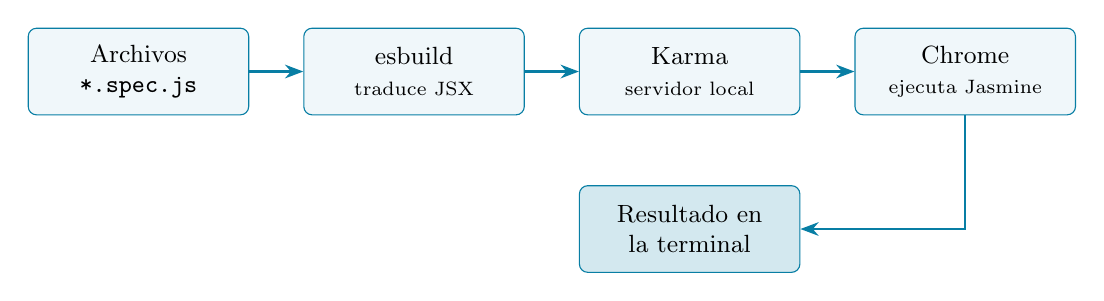
\begin{tikzpicture}[
  caja/.style={draw=reactblue, rounded corners=3pt, fill=reactblue!6, minimum width=2.8cm,
               minimum height=1.1cm, align=center, font=\small},
  flecha/.style={-{Stealth}, thick, reactblue}]
\node[caja] (spec) at (0,0) {Archivos\\\texttt{*.spec.js}};
\node[caja] (es)   at (3.5,0) {esbuild\\\scriptsize traduce JSX};
\node[caja] (k)    at (7,0) {Karma\\\scriptsize servidor local};
\node[caja] (ch)   at (10.5,0) {Chrome\\\scriptsize ejecuta Jasmine};
\node[caja, fill=reactblue!18] (t) at (7,-2) {Resultado en\\la terminal};
\draw[flecha] (spec) -- (es);
\draw[flecha] (es) -- (k);
\draw[flecha] (k) -- (ch);
\draw[flecha] (ch) |- (t);
\end{tikzpicture}
\end{center}

\begin{atencion}
El equipo de Karma anunció en 2023 que el proyecto está descontinuado: sigue funcionando, pero ya no recibe nuevas características. Muchos cursos y proyectos en producción lo siguen usando con Jasmine, y lo que aprendas aquí se traslada casi sin cambios a herramientas actuales como Vitest (sección \ref{sec:vitest}).
\end{atencion}

\subsection{Instalación y configuración}

\begin{terminal}
npm install -D karma karma-jasmine karma-chrome-launcher karma-esbuild jasmine-core
\end{terminal}

Necesitas Chrome instalado en el equipo. Agrega los scripts a \cmd{package.json}:
\begin{lstlisting}[language=JSX,numbers=none]
"scripts": {
  "test": "karma start",
  "test:watch": "karma start --no-single-run --auto-watch"
}
\end{lstlisting}

Crea el archivo de configuración en la raíz del proyecto:

\begin{lstlisting}[language=JSX,title={\small\ttfamily karma.conf.cjs}]
// Configuración de Karma. Usa .cjs porque package.json tiene "type": "module".
module.exports = function (config) {
  config.set({
    // Carpeta base desde donde se resuelven las rutas
    basePath: '',

    // Jasmine aporta describe, it, expect y los espías
    frameworks: ['jasmine'],

    // Archivos que Karma carga en el navegador
    files: [{ pattern: 'src/**/*.spec.js*', watched: false, type: 'module' }],

    // esbuild traduce JSX y resuelve los import antes de enviarlos al navegador
    preprocessors: { 'src/**/*.spec.js*': ['esbuild'] },

    esbuild: {
      target: 'es2022',
      jsx: 'automatic', // permite escribir JSX sin importar React
      loader: { '.js': 'jsx' },
    },

    // Cómo se muestran los resultados en la terminal
    reporters: ['progress'],

    // Navegador donde corren las pruebas. Chrome muestra la ventana;
    // ChromeHeadless corre sin interfaz, útil en servidores.
    browsers: ['ChromeHeadless'],

    // true: corre una vez y termina. false: queda esperando cambios.
    singleRun: true,
    autoWatch: false,

    port: 9876,
    colors: true,
    logLevel: config.LOG_INFO,
    concurrency: 1,
  })
}
\end{lstlisting}

Lo importante de ese archivo:
\begin{description}[leftmargin=0pt, style=nextline, itemsep=0.4em]
\item[\texttt{frameworks: ['jasmine']}] Carga Jasmine antes de tus pruebas, por eso \cmd{describe} e \cmd{it} existen sin importarlos.
\item[\texttt{files} y \texttt{preprocessors}] El patrón \cmd{src/**/*.spec.js*} toma todos los archivos que terminen en \cmd{.spec.js} o \cmd{.spec.jsx}, en cualquier subcarpeta de \cmd{src}. Cada uno pasa primero por esbuild.
\item[\texttt{esbuild.jsx: 'automatic'}] Permite escribir JSX en las pruebas de componentes sin importar React.
\item[\texttt{browsers}] \cmd{ChromeHeadless} corre Chrome sin abrir ventana. Usa \cmd{Chrome} si quieres ver el navegador y depurar con \cmd{F12}.
\item[\texttt{singleRun}] En \cmd{true} corre una vez y termina, que es lo que se usa al entregar o en un servidor de integración continua.
\end{description}

\begin{nota}
El nombre del archivo termina en \cmd{.cjs} porque \cmd{package.json} tiene \cmd{"type": "module"}. Con esa opción, todos los \cmd{.js} del proyecto se tratan como módulos ES, y Karma espera este archivo en el formato antiguo de Node.
\end{nota}

\subsection{Anatomía de una prueba}

\begin{lstlisting}[language=JSX]
describe('nombre del grupo', () => {   // agrupa pruebas relacionadas
  it('describe una conducta esperada', () => {
    const resultado = funcionQueSePrueba(entrada) // 1. preparar y ejecutar
    expect(resultado).toBe(valorEsperado)         // 2. comprobar
  })
})
\end{lstlisting}

\begin{itemize}
  \item \cmd{describe} agrupa. Se pueden anidar para organizar por función o por caso.
  \item \cmd{it} es una prueba. Su texto completa la frase ``it...'' (``debería...''), así que se escribe como una conducta: \emph{``suma uno por cada clic''}, no \emph{``prueba 1''}.
  \item \cmd{expect(...)} toma el valor obtenido y se compara con un \textbf{comparador} (\emph{matcher}).
\end{itemize}

Una forma útil de ordenar cada prueba es el patrón \textbf{preparar, ejecutar, comprobar}: primero los datos de entrada, después la llamada, al final las comprobaciones.

\subsection{Primer ejemplo}

\begin{lstlisting}[language=JSX,title={\small\ttfamily src/logica/formato.js}]
// Funciones puras: misma entrada, misma salida, sin tocar el DOM.
// Al estar separadas de los componentes se pueden probar con facilidad.

export function formatearPesos(valor) {
  return '$' + valor.toLocaleString('es-CL')
}

export function numeroAleatorio(maximo = 100) {
  return Math.floor(Math.random() * maximo) + 1
}
\end{lstlisting}
\begin{lstlisting}[language=JSX,title={\small\ttfamily src/logica/formato.spec.js}]
import { formatearPesos, numeroAleatorio } from './formato'

// describe agrupa pruebas relacionadas
describe('formatearPesos', () => {
  // it describe una conducta esperada, en una frase
  it('agrega el signo peso y separa los miles', () => {
    expect(formatearPesos(25990)).toBe('$25.990')
  })

  it('funciona con el cero', () => {
    expect(formatearPesos(0)).toBe('$0')
  })

  it('devuelve un texto', () => {
    expect(typeof formatearPesos(100)).toBe('string')
  })
})

describe('numeroAleatorio', () => {
  it('entrega un valor dentro del rango pedido', () => {
    for (let i = 0; i < 50; i++) {
      const n = numeroAleatorio(10)
      expect(n).toBeGreaterThanOrEqual(1)
      expect(n).toBeLessThanOrEqual(10)
    }
  })

  it('usa Math.random (espía)', () => {
    // El espía reemplaza a Math.random y siempre devuelve 0.5
    spyOn(Math, 'random').and.returnValue(0.5)
    expect(numeroAleatorio(100)).toBe(51)
    expect(Math.random).toHaveBeenCalled()
    expect(Math.random).toHaveBeenCalledTimes(1)
  })
})
\end{lstlisting}

El archivo de pruebas vive junto al que prueba y repite su nombre con \cmd{.spec} al medio. Así siempre se sabe qué está probado y qué no.

\subsection{Comparadores de Jasmine}

\begin{center}
\small
\begin{tabular}{>{\ttfamily}l p{9.3cm}}
\toprule
\textrm{\textbf{Comparador}} & \textbf{Comprueba que el valor} \\
\midrule
toBe(x) & Es idéntico a \cmd{x} (comparación \cmd{===}). Para números, textos y booleanos. \\
toEqual(x) & Tiene el mismo contenido que \cmd{x}. Para objetos y arreglos. \\
toBeTrue() / toBeFalse() & Es exactamente \cmd{true} o \cmd{false}. \\
toBeTruthy() / toBeFalsy() & Se evalúa como verdadero o falso. \\
toBeDefined() / toBeUndefined() & Existe o no existe. \\
toBeNull() & Es \cmd{null}. \\
toContain(x) & Contiene \cmd{x}, en un arreglo o en un texto. \\
toBeGreaterThan(n) & Es mayor que \cmd{n}. También existen \cmd{toBeLessThan} y las versiones \cmd{OrEqual}. \\
toBeCloseTo(n, d) & Se acerca a \cmd{n} con \cmd{d} decimales. Para cálculos con decimales. \\
toThrowError(msg) & Lanza un error con ese mensaje. Se usa con una función: \cmd{expect(() => f()).toThrowError()}. \\
toHaveBeenCalled() & Fue llamado. Solo para espías. \\
\bottomrule
\end{tabular}
\end{center}

Cualquier comparador se puede negar con \cmd{not}: \cmd{expect(x).not.toBe(3)}.

\begin{atencion}
\cmd{toBe} y \cmd{toEqual} no son lo mismo. \cmd{expect([1, 2]).toBe([1, 2])} falla, porque son dos arreglos distintos en memoria aunque tengan el mismo contenido. Con objetos y arreglos usa siempre \cmd{toEqual}.
\end{atencion}

\subsection{Preparar datos con \texttt{beforeEach}}

Cuando varias pruebas necesitan los mismos datos, se preparan en \cmd{beforeEach}, que se ejecuta antes de cada \cmd{it}. Así ninguna prueba hereda los cambios de la anterior.

\begin{lstlisting}[language=JSX,title={\small\ttfamily src/logica/cursos.spec.js}]
import { filtrarPorNombre, ordenarCursos } from './cursos'

describe('cursos', () => {
  let cursos

  // beforeEach corre antes de cada it: cada prueba parte con datos limpios
  beforeEach(() => {
    cursos = [
      { id: 1, nombre: 'Programación Web', creditos: 8 },
      { id: 2, nombre: 'Arquitectura de Software', creditos: 6 },
      { id: 3, nombre: 'Desarrollo Fullstack', creditos: 12 },
    ]
  })

  describe('filtrarPorNombre', () => {
    it('encuentra sin distinguir mayúsculas', () => {
      expect(filtrarPorNombre(cursos, 'DESARROLLO').length).toBe(1)
    })

    it('devuelve todos si la búsqueda está vacía', () => {
      expect(filtrarPorNombre(cursos, '   ').length).toBe(3)
    })

    it('devuelve un arreglo vacío si no hay coincidencias', () => {
      expect(filtrarPorNombre(cursos, 'química')).toEqual([])
    })
  })

  describe('ordenarCursos', () => {
    it('ordena alfabéticamente por nombre', () => {
      const nombres = ordenarCursos(cursos, 'nombre').map((c) => c.nombre)
      expect(nombres).toEqual(['Arquitectura de Software', 'Desarrollo Fullstack', 'Programación Web'])
    })

    it('ordena por créditos de mayor a menor', () => {
      expect(ordenarCursos(cursos, 'creditos')[0].creditos).toBe(12)
    })

    it('no modifica el arreglo original', () => {
      ordenarCursos(cursos, 'nombre')
      expect(cursos[0].nombre).toBe('Programación Web')
    })
  })
})
\end{lstlisting}

Jasmine ofrece cuatro ganchos: \cmd{beforeEach} y \cmd{afterEach} (antes y después de cada prueba) y \cmd{beforeAll} y \cmd{afterAll} (una vez por grupo).

\subsection{Probar los casos límite}

Los errores se esconden en los bordes: el cero, el arreglo vacío, el texto en blanco, el valor justo en el límite. En una escala de 1 a 7 con 4 como nota mínima, hay que probar 3,9 y 4,0.

\begin{lstlisting}[language=JSX,title={\small\ttfamily src/logica/notas.spec.js}]
import { estaAprobado, mensajePara, NOTA_MINIMA } from './notas'

describe('estaAprobado', () => {
  it('aprueba desde la nota mínima', () => {
    expect(estaAprobado(NOTA_MINIMA)).toBeTrue()
    expect(estaAprobado(4.0)).toBeTrue()
  })

  it('reprueba bajo la nota mínima', () => {
    expect(estaAprobado(3.9)).toBeFalse()
  })
})

describe('mensajePara', () => {
  // Los casos límite son los que más errores descubren
  const casos = [
    { nota: 7.0, esperado: 'Excelente' },
    { nota: 6.0, esperado: 'Excelente' },
    { nota: 5.9, esperado: 'Aprobado' },
    { nota: 4.0, esperado: 'Aprobado' },
    { nota: 3.9, esperado: 'Reprobado' },
    { nota: 1.0, esperado: 'Reprobado' },
  ]

  casos.forEach(({ nota, esperado }) => {
    it(`con nota ${nota} devuelve "${esperado}"`, () => {
      expect(mensajePara(nota)).toBe(esperado)
    })
  })
})
\end{lstlisting}

Como \cmd{it} es una función normal, se puede llamar dentro de un \cmd{forEach} para generar una prueba por caso sin repetir código.

\subsection{Separar la lógica de la interfaz}

Una función que solo recibe datos y devuelve datos se prueba en una línea. Un componente, en cambio, necesita un navegador, un contenedor y simulación de clics. Por eso conviene sacar las reglas del negocio del componente y dejarlas en funciones puras.

En el proyecto de acompañamiento, la carpeta \cmd{src/logica/} contiene todo lo que se puede probar sin navegador:

\begin{center}
\small
\begin{tabular}{>{\ttfamily}l p{8.7cm}}
\toprule
\textrm{\textbf{Archivo}} & \textbf{Qué contiene} \\
\midrule
formato.js & Formato de precios y número aleatorio. \\
seguridad.js & Nivel de seguridad de una contraseña. \\
notas.js & Aprobación y mensaje según la nota. \\
cursos.js & Filtrar y ordenar cursos. \\
inscripcion.js & Validación del formulario. \\
tareas.js & Crear, agregar, alternar, eliminar y contar tareas. \\
api.js & Obtener títulos desde la API. \\
\bottomrule
\end{tabular}
\end{center}

El componente queda más corto y se limita a mostrar:
\begin{lstlisting}[language=JSX]
// Antes: la regla estaba escrita dentro del componente
let seguridad = 'Debil'
if (clave.length >= 8 && /\d/.test(clave)) seguridad = 'Fuerte'
else if (clave.length >= 6) seguridad = 'Media'

// Despues: la regla vive en src/logica/seguridad.js y tiene sus pruebas
const seguridad = nivelSeguridad(clave)
\end{lstlisting}

\subsection{Espías}

Un \textbf{espía} (\emph{spy}) reemplaza una función para observar cómo se usó o para controlar lo que devuelve. Sirve cuando el código depende de algo impredecible (el azar, la hora) o costoso (la red).

\begin{lstlisting}[language=JSX]
spyOn(Math, 'random').and.returnValue(0.5) // reemplaza y fija el resultado
spyOn(objeto, 'metodo').and.callThrough()  // observa sin cambiar la conducta
spyOn(objeto, 'metodo').and.callFake(fn)   // lo reemplaza por otra funcion
const espia = jasmine.createSpy('nombre')  // una funcion falsa desde cero

expect(espia).toHaveBeenCalled()
expect(espia).toHaveBeenCalledTimes(2)
expect(espia).toHaveBeenCalledWith('Leer')
espia.calls.mostRecent().args // argumentos de la ultima llamada
\end{lstlisting}

Los espías creados con \cmd{spyOn} se deshacen solos al terminar cada prueba.

\subsection{Pruebas asíncronas}

Para probar código que espera una respuesta, la función del \cmd{it} se declara \cmd{async} y se usa \cmd{await}. En lugar de salir a internet, se le entrega a la función una versión falsa de \cmd{fetch}: la prueba queda rápida y su resultado no depende de la conexión.

\begin{lstlisting}[language=JSX,title={\small\ttfamily src/logica/api.js}]
// El segundo parámetro permite reemplazar fetch por una función falsa en las pruebas.
export async function obtenerTitulos(usuarioId, traer = fetch) {
  const res = await traer(`https://jsonplaceholder.typicode.com/posts?userId=${usuarioId}`)
  if (!res.ok) throw new Error('Error ' + res.status)
  const datos = await res.json()
  return datos.map((p) => p.title)
}
\end{lstlisting}
\begin{lstlisting}[language=JSX,title={\small\ttfamily src/logica/api.spec.js}]
import { obtenerTitulos } from './api'

describe('obtenerTitulos', () => {
  it('devuelve solo los títulos', async () => {
    // Doble de prueba: imita la respuesta de fetch sin salir a internet
    const traerFalso = jasmine.createSpy('traer').and.returnValue(
      Promise.resolve({
        ok: true,
        json: () => Promise.resolve([{ title: 'uno' }, { title: 'dos' }]),
      }),
    )

    const titulos = await obtenerTitulos(3, traerFalso)

    expect(titulos).toEqual(['uno', 'dos'])
    expect(traerFalso).toHaveBeenCalledTimes(1)
    // Se revisa que la URL incluya el usuario pedido
    expect(traerFalso.calls.mostRecent().args[0]).toContain('userId=3')
  })

  it('lanza un error si la respuesta falla', async () => {
    const traerFalso = () => Promise.resolve({ ok: false, status: 404 })
    await expectAsync(obtenerTitulos(1, traerFalso)).toBeRejectedWithError('Error 404')
  })
})
\end{lstlisting}

\cmd{expectAsync} es la versión de \cmd{expect} para promesas. Sus comparadores son \cmd{toBeResolved}, \cmd{toBeResolvedTo}, \cmd{toBeRejected} y \cmd{toBeRejectedWithError}.

\subsection{Probar un componente}

Para probar un componente hay que montarlo en un contenedor, provocar la interacción y revisar lo que quedó en pantalla. \cmd{act} agrupa cada acción y espera a que React termine de renderizar antes de continuar.

\begin{lstlisting}[language=JSX,title={\small\ttfamily src/components/basicos/Contador.spec.jsx}]
import { act } from 'react'
import { createRoot } from 'react-dom/client'
import Contador from './Contador'

// React necesita saber que está en un entorno de pruebas
globalThis.IS_REACT_ACT_ENVIRONMENT = true

describe('Contador (componente)', () => {
  let contenedor
  let raiz

  beforeEach(() => {
    contenedor = document.createElement('div')
    document.body.appendChild(contenedor)
    raiz = createRoot(contenedor)
  })

  afterEach(() => {
    // Limpieza: cada prueba debe partir con la pantalla vacía
    act(() => raiz.unmount())
    contenedor.remove()
  })

  const renderizar = () => act(() => raiz.render(<Contador />))
  const clicEn = (boton) => act(() => boton.dispatchEvent(new MouseEvent('click', { bubbles: true })))

  it('parte en cero', () => {
    renderizar()
    expect(contenedor.textContent).toContain('Has hecho clic 0 veces')
  })

  it('suma uno por cada clic', () => {
    renderizar()
    const sumar = contenedor.querySelectorAll('button')[0]
    clicEn(sumar)
    clicEn(sumar)
    expect(contenedor.textContent).toContain('Has hecho clic 2 veces')
  })

  it('vuelve a cero con el botón Reiniciar', () => {
    renderizar()
    const [sumar, reiniciar] = contenedor.querySelectorAll('button')
    clicEn(sumar)
    clicEn(reiniciar)
    expect(contenedor.textContent).toContain('Has hecho clic 0 veces')
  })
})
\end{lstlisting}

\begin{description}[leftmargin=0pt, style=nextline, itemsep=0.4em]
\item[\texttt{IS\_REACT\_ACT\_ENVIRONMENT}] Le indica a React que está en pruebas. Sin esta línea aparece una advertencia en consola.
\item[\texttt{beforeEach} y \texttt{afterEach}] Crean y destruyen el contenedor. Sin la limpieza, los componentes de una prueba quedarían en la página durante la siguiente.
\item[\texttt{contenedor.textContent}] Es el texto visible. Se comprueba lo que ve el usuario, no cómo está implementado el componente por dentro.
\item[\texttt{dispatchEvent}] Simula el clic. La opción \cmd{bubbles: true} es necesaria porque React escucha los eventos en la raíz.
\end{description}

\begin{nota}
La biblioteca \textbf{React Testing Library} hace esto mismo con menos código (\cmd{render}, \cmd{screen.getByText}, \cmd{fireEvent.click}) y es el estándar actual para probar componentes. Vale la pena mirarla después de entender lo que ocurre por debajo.
\end{nota}

\subsection{Ejecutar las pruebas}

\begin{terminal}
npm test          # corre todo una vez y muestra el resumen
npm run test:watch  # queda escuchando y repite al guardar
\end{terminal}

La salida indica cuántas pruebas pasaron y detalla las que fallaron con el valor esperado y el obtenido:
\begin{terminal}
Chrome Headless 140.0.0: Executed 44 of 44 SUCCESS (0.35 secs / 0.29 secs)
\end{terminal}

Mientras escribes una prueba puedes enfocarte en una sola: \cmd{fit} y \cmd{fdescribe} ejecutan únicamente esa prueba o ese grupo; \cmd{xit} y \cmd{xdescribe} los saltan. Recuerda devolverlos a \cmd{it} y \cmd{describe} antes de entregar.

\begin{atencion}
Si aparece \emph{No binary for ChromeHeadless browser}, Karma no encontró Chrome. Indícale la ruta con la variable \cmd{CHROME\_BIN}:\\
Windows (PowerShell):\\
\mbox{\footnotesize\cmd{\$env:CHROME\_BIN="C:\textbackslash Program Files\textbackslash Google\textbackslash Chrome\textbackslash Application\textbackslash chrome.exe"}}\\
Linux: \cmd{export CHROME\_BIN=\$(which google-chrome)}
\end{atencion}

\subsection{Errores frecuentes al probar}

\begin{center}
\small
\begin{tabular}{p{5.4cm} p{8.6cm}}
\toprule
\textbf{Síntoma} & \textbf{Causa y solución} \\
\midrule
\emph{Expected [1, 2] to be [1, 2]} & Usaste \cmd{toBe} con un arreglo u objeto. Cambia a \cmd{toEqual}. \\
\addlinespace
La prueba pasa sola pero falla junto a otras & Alguna prueba modifica datos compartidos. Crea los datos dentro de \cmd{beforeEach}. \\
\addlinespace
\emph{Executed 0 of 0} & Ningún archivo coincide con el patrón de \cmd{files}. Revisa el nombre \cmd{.spec.js}. \\
\addlinespace
La prueba asíncrona pasa siempre & Olvidaste \cmd{await} o marcar la función como \cmd{async}. \\
\addlinespace
\emph{An update to X inside a test was not wrapped in act} & Falta envolver la interacción en \cmd{act(...)}. \\
\addlinespace
La prueba se rompe al cambiar el diseño & Estás comprobando detalles internos. Compara el texto visible. \\
\bottomrule
\end{tabular}
\end{center}

\subsection{Buenas prácticas}

\begin{itemize}
  \item Una conducta por prueba. Si el nombre necesita un ``y'', probablemente son dos pruebas.
  \item Cada prueba debe poder correr sola y en cualquier orden.
  \item Prueba lo que hace tu código, no lo que hace React ni otras bibliotecas.
  \item Cuando aparezca un error, escribe primero una prueba que lo reproduzca y después corrígelo. Esa prueba evita que el error vuelva.
  \item Mide la cobertura si quieres, pero recuerda que un 100\% no garantiza que las comprobaciones sean buenas.
\end{itemize}

\subsection{La alternativa actual: Vitest}\label{sec:vitest}

Vitest usa la misma configuración de Vite, no necesita navegador y su sintaxis es casi idéntica:
\begin{terminal}
npm install -D vitest jsdom @testing-library/react
\end{terminal}
\begin{lstlisting}[language=JSX]
import { describe, it, expect } from 'vitest' // en Jasmine son globales
import { mensajePara } from './notas'

describe('mensajePara', () => {
  it('aprueba con 4.0', () => {
    expect(mensajePara(4.0)).toBe('Aprobado') // identico a Jasmine
  })
})
\end{lstlisting}

Los cambios principales son que las funciones se importan, que los espías se crean con \cmd{vi.fn()} y \cmd{vi.spyOn()}, y que se ejecuta con \cmd{npx vitest}. Todo lo aprendido sobre qué probar sigue igual.

\begin{ejercicio}[de pruebas 1]
Escribe \cmd{src/logica/carrito.js} con las funciones \cmd{agregarProducto}, \cmd{quitarProducto} y \cmd{totalCarrito}, y su archivo de pruebas. Incluye el caso del carrito vacío.
\end{ejercicio}

\begin{ejercicio}[de pruebas 2]
Rompe a propósito \cmd{nivelSeguridad}, cambiando el 8 por un 4, y ejecuta \cmd{npm test}. Observa qué prueba falla y qué mensaje entrega. Esa es la utilidad real de tener pruebas.
\end{ejercicio}

\begin{ejercicio}[de pruebas 3]
Escribe las pruebas del componente \cmd{Interruptor}: que el texto esté oculto al inicio, que aparezca con el primer clic y que desaparezca con el segundo.
\end{ejercicio}


%=====================================================
\section{Generar la versión de producción}

Cuando la aplicación esté lista:
\begin{terminal}
npm run build
npm run preview
\end{terminal}

\cmd{build} crea la carpeta \cmd{dist/} con archivos HTML, CSS y JavaScript optimizados. Ese contenido se puede publicar gratis en servicios como Netlify, Vercel o GitHub Pages.

\begin{nota}
Antes de subir el proyecto a GitHub, verifica que \cmd{.gitignore} incluya \cmd{node\_modules} y \cmd{dist}. Vite ya lo trae configurado. Quien clone el repositorio solo debe ejecutar \cmd{npm install}.
\end{nota}

%=====================================================
\section{Errores frecuentes}

\begin{center}
\small
\begin{tabular}{p{5.6cm} p{8.6cm}}
\toprule
\textbf{Síntoma} & \textbf{Causa y solución} \\
\midrule
\emph{Adjacent JSX elements must be wrapped} & Devuelves varios elementos sin padre. Envuélvelos en \cmd{<>...</>}. \\
\addlinespace
El componente no aparece o sale como etiqueta HTML & El nombre empieza con minúscula. Usa \cmd{Tarjeta}, no \cmd{tarjeta}. \\
\addlinespace
\emph{Each child in a list should have a unique key} & Falta \cmd{key} en los elementos del \cmd{map}. \\
\addlinespace
\emph{Too many re-renders} & Llamas una función en vez de pasarla: \cmd{onClick=\{f()\}}. Cambia a \cmd{onClick=\{f\}} o \cmd{onClick=\{() => f(x)\}}. \\
\addlinespace
La pantalla no cambia al modificar datos & Modificaste el estado directamente (\cmd{push}, asignación). Crea un arreglo u objeto nuevo y usa \cmd{set}. \\
\addlinespace
\emph{Failed to resolve import} & Ruta o nombre de archivo mal escrito. Revisa mayúsculas y la extensión. \\
\addlinespace
\emph{Port 5173 is in use} & Hay otro servidor corriendo. Ciérralo o acepta el puerto alternativo que propone Vite. \\
\addlinespace
El input no deja escribir & Tiene \cmd{value} pero no \cmd{onChange}. \\
\bottomrule
\end{tabular}
\end{center}

%=====================================================
\section{Resumen de comandos}

\begin{terminal}
node -v                                   # version de Node
npm -v                                    # version de npm
npm create vite@latest app -- --template react
cd app
npm install                               # instala dependencias
npm run dev                               # servidor de desarrollo
npm install nombre-paquete                # agrega una libreria
npm test                                  # pruebas unitarias
npm run build                             # version de produccion
npm run preview                           # prueba la version final
\end{terminal}

%=====================================================
\section{Glosario}

\begin{center}
\small
\begin{tabular}{>{\bfseries}p{3.4cm} p{10.2cm}}
\toprule
Término & Significado \\
\midrule
Componente & Función que devuelve JSX. Su nombre empieza con mayúscula. \\
JSX & Sintaxis parecida a HTML que se escribe dentro de JavaScript. \\
Props & Datos que un componente recibe de su padre. Son de solo lectura. \\
children & Prop especial con el contenido escrito entre las etiquetas del componente. \\
Estado & Datos que un componente recuerda y que, al cambiar, provocan un nuevo render. \\
Valor derivado & Dato que se calcula a partir del estado o de las props en cada render. \\
Hook & Función de React que empieza con \cmd{use} (\cmd{useState}, \cmd{useEffect}). \\
Render & Ejecución de la función del componente para obtener su JSX. \\
Commit & Fase en que React aplica al DOM las diferencias encontradas. \\
Montar / desmontar & Aparecer en pantalla por primera vez / ser eliminado de ella. \\
Efecto & Código que sincroniza el componente con algo externo a React. \\
DOM & Árbol de objetos que el navegador construye a partir del HTML. \\
SPA & Aplicación de una sola página cuyo contenido cambia con JavaScript. \\
key & Identificador único de cada elemento de una lista. \\
Input controlado & Campo cuyo valor está guardado en el estado. \\
Fragmento & \cmd{<>...</>}: agrupa elementos sin agregar etiquetas al DOM. \\
Paquete & Biblioteca instalada con npm. Se registra en \cmd{package.json}. \\
Levantar el estado & Mover el estado al padre común de los componentes que lo necesitan. \\
\bottomrule
\end{tabular}
\end{center}


%=====================================================
\section{Próximos pasos}

Con lo visto ya puedes construir aplicaciones de una sola vista. El orden sugerido para seguir avanzando es:

\begin{enumerate}[leftmargin=*]
  \item \textbf{React Router}: navegación entre páginas (\cmd{npm install react-router}).
  \item \textbf{Hooks adicionales}: \cmd{useRef}, \cmd{useContext} para compartir datos sin pasar props por muchos niveles, y \cmd{useReducer} para estados complejos.
  \item \textbf{Hooks personalizados}: extraer lógica repetida, por ejemplo un \cmd{useFetch}.
  \item \textbf{Estilos}: Tailwind CSS o CSS Modules.
  \item \textbf{TypeScript}: tipar props y estado. Se crea con la plantilla \cmd{react-ts}.
  \item \textbf{Pruebas de componentes}: React Testing Library, sobre lo visto en la sección \ref{sec:pruebas}.
  \item \textbf{Frameworks}: Next.js o React Router en modo framework, para renderizado en servidor.
\end{enumerate}

\textbf{Documentación oficial:} \url{https://react.dev/learn}. Está disponible en español en \url{https://es.react.dev} e incluye ejercicios interactivos al final de cada tema.

\end{document}
